%\documentclass[handout]{beamer}
\documentclass{beamer}
\usepackage{setspace}
\usepackage{sansmathaccent}
\pdfmapfile{+sansmathaccent.map}

\usepackage{tikz}
\definecolor{homepage}{RGB}{2,213,206}
\definecolor{cblue}{RGB}{217,243,253}
\definecolor{alertred}{RGB}{180,30,30}

\usepackage{amsmath,amsthm,amssymb,beamerthemesplit,multimedia,hyperref,graphicx,booktabs,array}
\usetikzlibrary{shapes.geometric, arrows}

\newcommand{\R}{\mathbb{R}}
\newcommand{\E}{\mathbb{E}}
\newcommand{\half}{\tfrac{1}{2}}

\usetheme{Frankfurt}
\usecolortheme{beaver}

\title{The Sperm Parasite Paradox}
\subtitle{Stochastic Stabilization in Gynogenetic Complexes}
\author{Prof.\ Juan B.\ Gutiérrez}
\institute[UTSA]{\textsc{The University of Texas at San Antonio}}
\date{\footnotesize Texas Differential Equations Conference 2026}
\setbeamertemplate{footline}[page number]{}

\begin{document}

%%-------------------------------------------------
%% SLIDE 1: Title
%%-------------------------------------------------
\begin{frame}
  \titlepage
  \vspace{-0.4cm}
  \begin{center}
    \footnotesize \texttt{juan.gutierrez3@utsa.edu}
  \end{center}
\end{frame}

%%-------------------------------------------------
\section{Biology}
\stepcounter{subsection}
%%-------------------------------------------------

%%-------------------------------------------------
%% SLIDE 2: The Paradox
%%-------------------------------------------------
\begin{frame}{The Sperm Parasite Paradox}

  \begin{columns}[T]
    \begin{column}{0.55\textwidth}
      \textbf{The logic of collapse:}
      \begin{enumerate}
        \item Each male--parasite mating produces \emph{only} parasite offspring
        \item Growing parasite population diverts male effort from host females
        \item Fewer host matings $\Rightarrow$ fewer males next generation
        \item Fewer males $\Rightarrow$ less sperm for everyone
        \item Positive feedback $\Rightarrow$ \textbf{extinction}
      \end{enumerate}

      \vspace{0.4cm}
      \textbf{Yet:} \textit{Poecilia formosa} has coexisted with
      \textit{P.~mexicana} and \textit{P.~latipinna} for
      $\mathbf{> 100{,}000}$ \textbf{years}~\textit{(Avise 1991)}.

      \vspace{0.3cm}
      \textcolor{alertred}{\textbf{How?}}
    \end{column}

    \begin{column}{0.45\textwidth}
      \vspace{0.2cm}
      \begin{block}{Key biology}
        \textit{P.~formosa} = \textbf{sperm parasite}\\[4pt]
        Requires host male sperm to\\
        trigger embryogenesis\\[4pt]
        Paternal genome \textbf{excluded}\\
        from all offspring\\[4pt]
        All-female species: 100\%\\
        parasite daughters
      \end{block}
    \end{column}
  \end{columns}

\end{frame}

%%-------------------------------------------------
%% SLIDE 3: Field Evidence
%%-------------------------------------------------
\begin{frame}{Field Evidence: Behavioral Discrimination}

  \footnotesize

  \begin{columns}[T]
    \begin{column}{0.52\textwidth}
      \textbf{Riesch, Schlupp \& Plath (2008):}\\
      Sperm acquisition in natural populations
      of \textit{P.~latipinna} + \textit{P.~formosa}

      \vspace{0.3cm}
      \begin{tabular}{lcc}
        \toprule
        Species & \% with sperm \\
        \midrule
        Host females & \textbf{74\%} \\
        Parasite females & \textbf{10\%} \\
        \bottomrule
      \end{tabular}

      \vspace{0.4cm}
      \begin{itemize}
        \item Discrimination is \textbf{behavioral}, not physiological
        \item Males allocate sperm \emph{actively}
        \item Discrimination persists even when males are exceedingly rare
        \item Fecundity of lab-reared \textit{P.~formosa} is normal when sperm is given
      \end{itemize}
    \end{column}

    \begin{column}{0.48\textwidth}
      \vspace{0.1cm}
      \begin{block}{Mechanism}
        Upon each parasite encounter, \\
        host male accepts with probability
        $\gamma \in (0,1]$\\[6pt]
        $\gamma$ = \textbf{per-encounter acceptance\\
        probability}\\[6pt]
        Not a vague ``discrimination factor''---\\
        a measurable behavioral parameter
      \end{block}

      \vspace{0.2cm}
      \begin{block}{Environmental context}
        Soto La Marina drainage: seasonal\\
        flooding, pool isolation/reconnection\\[4pt]
        High year-to-year variation in\\
        parasite proportion $\Rightarrow$\\
        \textbf{stochastic forcing is real}
      \end{block}
    \end{column}
  \end{columns}

\end{frame}

%%-------------------------------------------------
%% SLIDE 4: Prior Models and Their Gaps
%%-------------------------------------------------
\begin{frame}{Prior Models: What Is Missing}
  \footnotesize

  \begin{tabular}{p{2.1cm}p{3.1cm}p{4.1cm}}
    \toprule
    \textbf{Study} & \textbf{Contribution} & \textbf{Gap} \\
    \midrule
    Kiester (1981) & Discrimination necessary for persistence & Fixed $\gamma$; no 3-population structure \\[4pt]
    Schley (2004) & Ecological factors + Allee effects & No parasitism \\[4pt]
    Peck (1999) & Spatial fragmentation matters & No discrimination behavior \\[4pt]
    Kokko (2008) & Spatial dynamics + sperm limitation & $\gamma$ not population-dependent \\[4pt]
    Heubel (2009) & Male efficiency + fixed discrimination & Fixed $\gamma$; no stochasticity \\
    \bottomrule
  \end{tabular}

  \vspace{0.4cm}
  \textbf{Common gaps in all prior models:}
  \begin{itemize}
    \item No population-\emph{dependent} discrimination function $\gamma(p)$
    \item No systematic comparison of competing stochastic formulations
    \item Discrimination \emph{speed} never identified as the key control variable
  \end{itemize}

\end{frame}

%%-------------------------------------------------
\section{Model}
\stepcounter{subsection}
%%-------------------------------------------------

%%-------------------------------------------------
%% SLIDE 5: Three Populations — Mechanistic Derivation
%%-------------------------------------------------
\begin{frame}{Mechanistic Derivation: Two Steps}
  \footnotesize

  \textbf{State:} host females $f$, host males $m$, parasite females $p$

  \vspace{0.3cm}
  \begin{columns}[T]
    \begin{column}{0.5\textwidth}
      \textbf{Step 1 — Per-encounter acceptance}\\[4pt]
      Mass-action encounters; upon each\\
      parasite encounter, male accepts\\
      with probability $\gamma$:
      \begin{align*}
        \text{host matings:}    &\;\alpha\,m\,f \\
        \text{parasite matings:}&\;\gamma\,\alpha\,m\,p
      \end{align*}
      Independent pools at this stage.\\[8pt]

      \textbf{Step 2 — Finite mating capacity}\\[4pt]
      Each accepted parasite mating\\
      \emph{displaces} one host-female mating:
      \[
        \alpha m f - \gamma\alpha m p
        = \alpha m(f - \gamma p)
      \]
    \end{column}

    \begin{column}{0.5\textwidth}
      \begin{alertblock}{Key result}
        $m(f - \gamma p)$ is a \textbf{theorem}\\
        of Steps 1 \& 2, not an assumption.\\[6pt]
        Critics of the functional form\\
        must challenge Step 2 specifically:\\
        \emph{Is male mating capacity finite?}\\[6pt]
        Riesch (2008): yes --- sperm\\
        allocation is a zero-sum budget.
      \end{alertblock}

      \vspace{0.2cm}
      \textit{Simplifying assumption:}\\
      Displacement coefficient $c=1$\\
      (future: calibrate from sperm-count data)
    \end{column}
  \end{columns}

\end{frame}

%%-------------------------------------------------
%% SLIDE 6: The ODE System
%%-------------------------------------------------
\begin{frame}{The Deterministic System}
  \footnotesize

  \textbf{Dimensional system} (tildes = dimensional quantities):
  \begin{align*}
    \frac{d\tilde{f}}{dt} &=
      a\,\tilde{\beta}\,\tilde{L}\,\tilde{m}(\tilde{f}-\gamma\tilde{p})
      - \tilde{\delta}\,\tilde{f} \\[4pt]
    \frac{d\tilde{m}}{dt} &=
      (1-a)\,\tilde{\beta}\,\tilde{L}\,\tilde{m}(\tilde{f}-\gamma\tilde{p})
      - \tilde{\delta}\,\tilde{m} \\[4pt]
    \frac{d\tilde{p}}{dt} &=
      \gamma\,\tilde{\beta}\,\tilde{L}\,\tilde{m}\,\tilde{p}
      - \tilde{\delta}\,\tilde{p}
  \end{align*}
  where $\tilde{L} = 1 - (\tilde{f}+\tilde{m}+\tilde{p})/\tilde{K}$

  \vspace{0.3cm}
  \textbf{Non-dimensionalize:} $u_i = \tilde{u}_i/\tilde{K}$,
  $\tau = \tilde{\delta}\,t$, $\beta = \tilde{\beta}\tilde{K}/\tilde{\delta}$

  \vspace{0.2cm}
  \begin{center}
  \begin{tabular}{llll}
    \toprule
    Parameter & Symbol & Value & Source \\
    \midrule
    Birth rate (nondim) & $\beta$ & 300 & $0.1 \times 300 / 0.1$ \\
    Female fraction & $a$ & 0.8 & Balsano (1989) \\
    Carrying capacity & $\tilde{K}$ & 300 & field estimate \\
    Discrim.\ (initial) & $\gamma_o$ & 1.0 & no preference \\
    Discrim.\ (asymp.) & $\gamma_\infty$ & 0.2 & Riesch (2008) \\
    \bottomrule
  \end{tabular}
  \end{center}

\end{frame}

%%-------------------------------------------------
%% SLIDE 7: Discrimination Function
%%-------------------------------------------------
\begin{frame}{Population-Dependent Discrimination $\gamma(p)$}

    \footnotesize

  \begin{columns}[T]
    \begin{column}{0.48\textwidth}
      Sigmoid function:
      \[
        \gamma(p) = \frac{\gamma_o - \gamma_\infty}{1+e^{vp-r}} + \gamma_\infty
      \]
      \begin{itemize}
        \item $\gamma_o = 1$: no preference when parasites rare
        \item $\gamma_\infty = 0.2$: strong discrimination when parasites common
        \item $v > 0$: \textbf{speed of discrimination}
        \item $r = 5$: sigmoid shift
      \end{itemize}

      \vspace{0.3cm}
      \textbf{$v$ is the pivotal parameter:}\\
      slow $v$ $\Rightarrow$ extinction\\
      fast $v$ $\Rightarrow$ coexistence
    \end{column}

    \begin{column}{0.52\textwidth}
      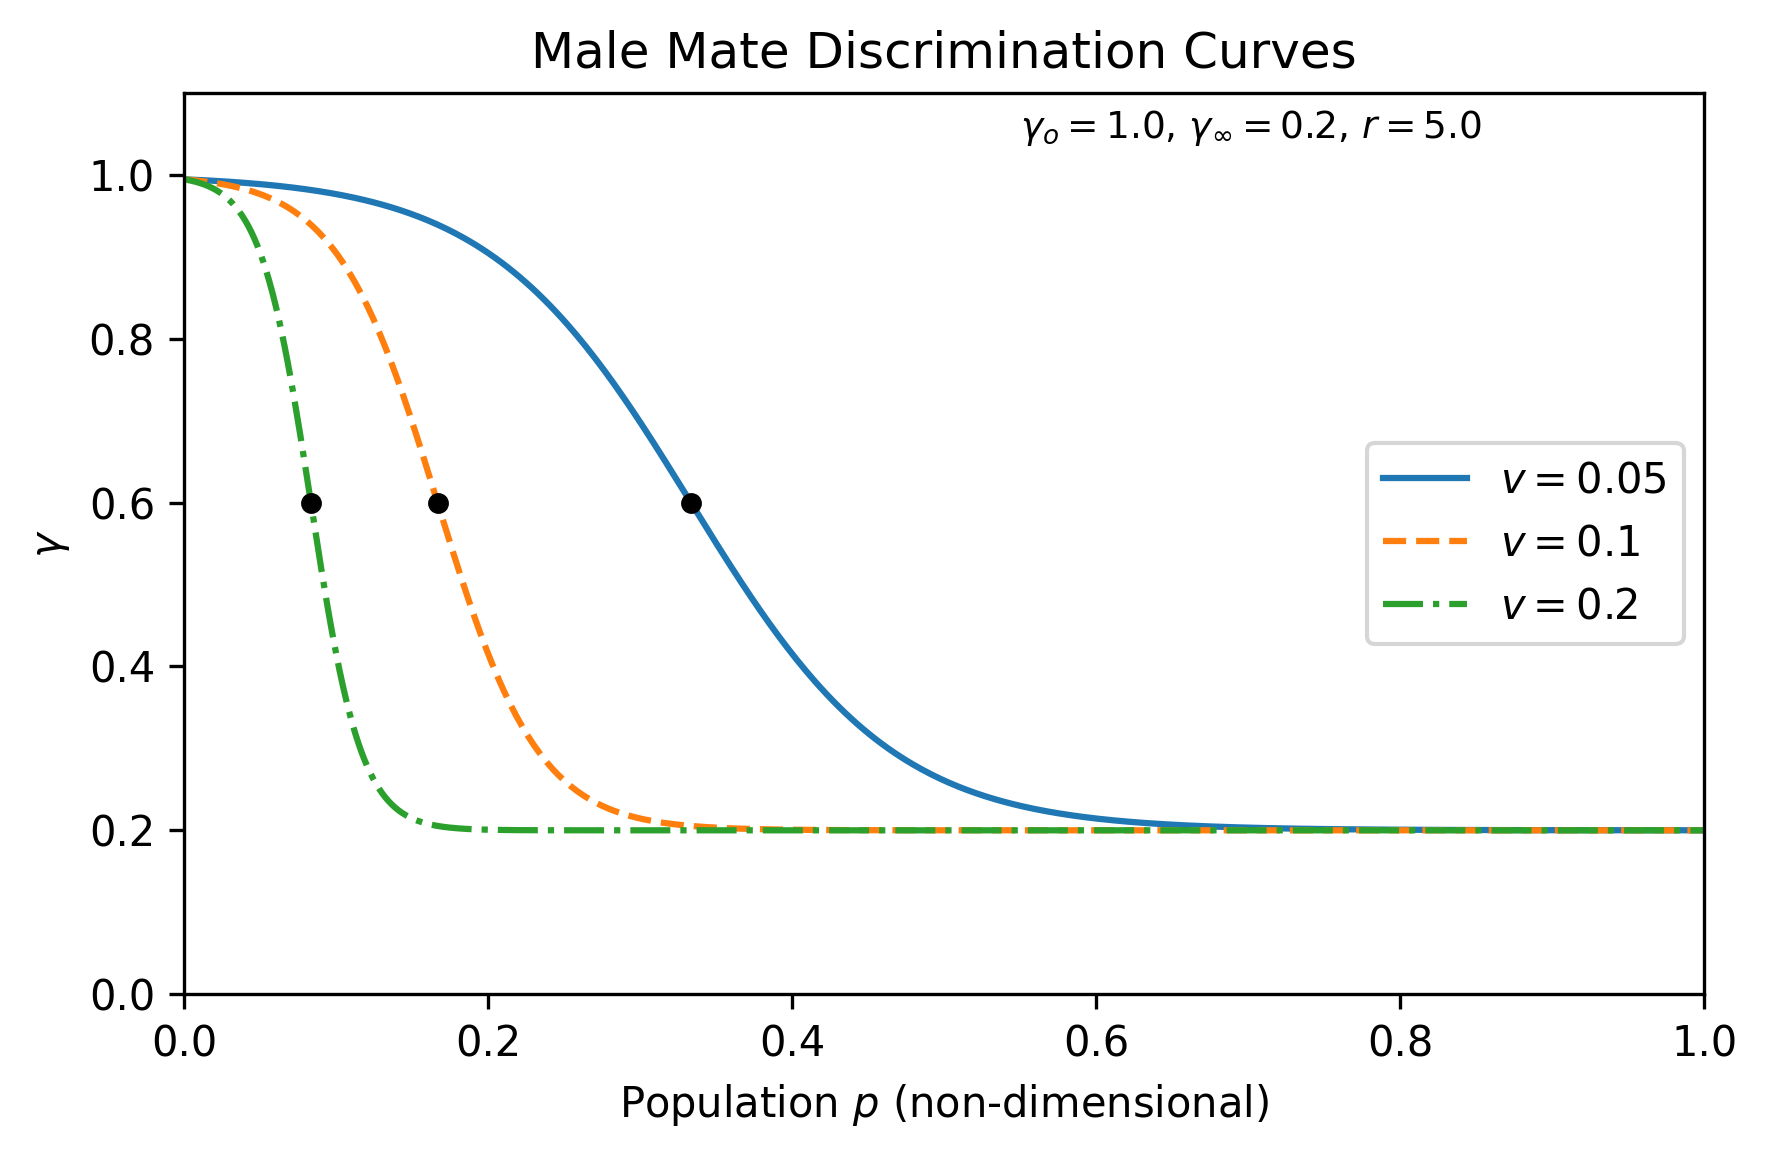
\includegraphics[width=\linewidth]{../poecilia_sde/figures/fig01_gamma_curves.png}
      {\tiny Three discrimination speeds. Black dots: inflection points.}
    \end{column}
  \end{columns}

\end{frame}

%%-------------------------------------------------
%% SLIDE 8: Deterministic Fate — Extinction
%%-------------------------------------------------
\begin{frame}{Deterministic Fate: Extinction Without Noise}

  \footnotesize
  \begin{columns}[T]
    \begin{column}{0.48\textwidth}
      \textbf{Equilibrium condition:}
      \[
        \gamma_{eq} = \frac{a\,f^*}{a\,p^* + f^*} \approx 0.74
      \]

      Three regimes:
      \begin{itemize}
        \item $\gamma < \gamma_{eq}$: \textcolor{alertred}{\textbf{extinction}}
        \item $\gamma = \gamma_{eq}$: coexistence
        \item $\gamma > \gamma_{eq}$: parasites extinct, hosts recover
      \end{itemize}

      \vspace{0.3cm}
      Slow discrimination ($v=6$, nondim):
      parasite initially grows, draws down\\
      host males, starves host females,\\
      eventually collapses itself.

      \vspace{0.2cm}
      \textbf{Without noise: no escape.}\\
      \textbf{With noise: ?}
    \end{column}

    \begin{column}{0.52\textwidth}
      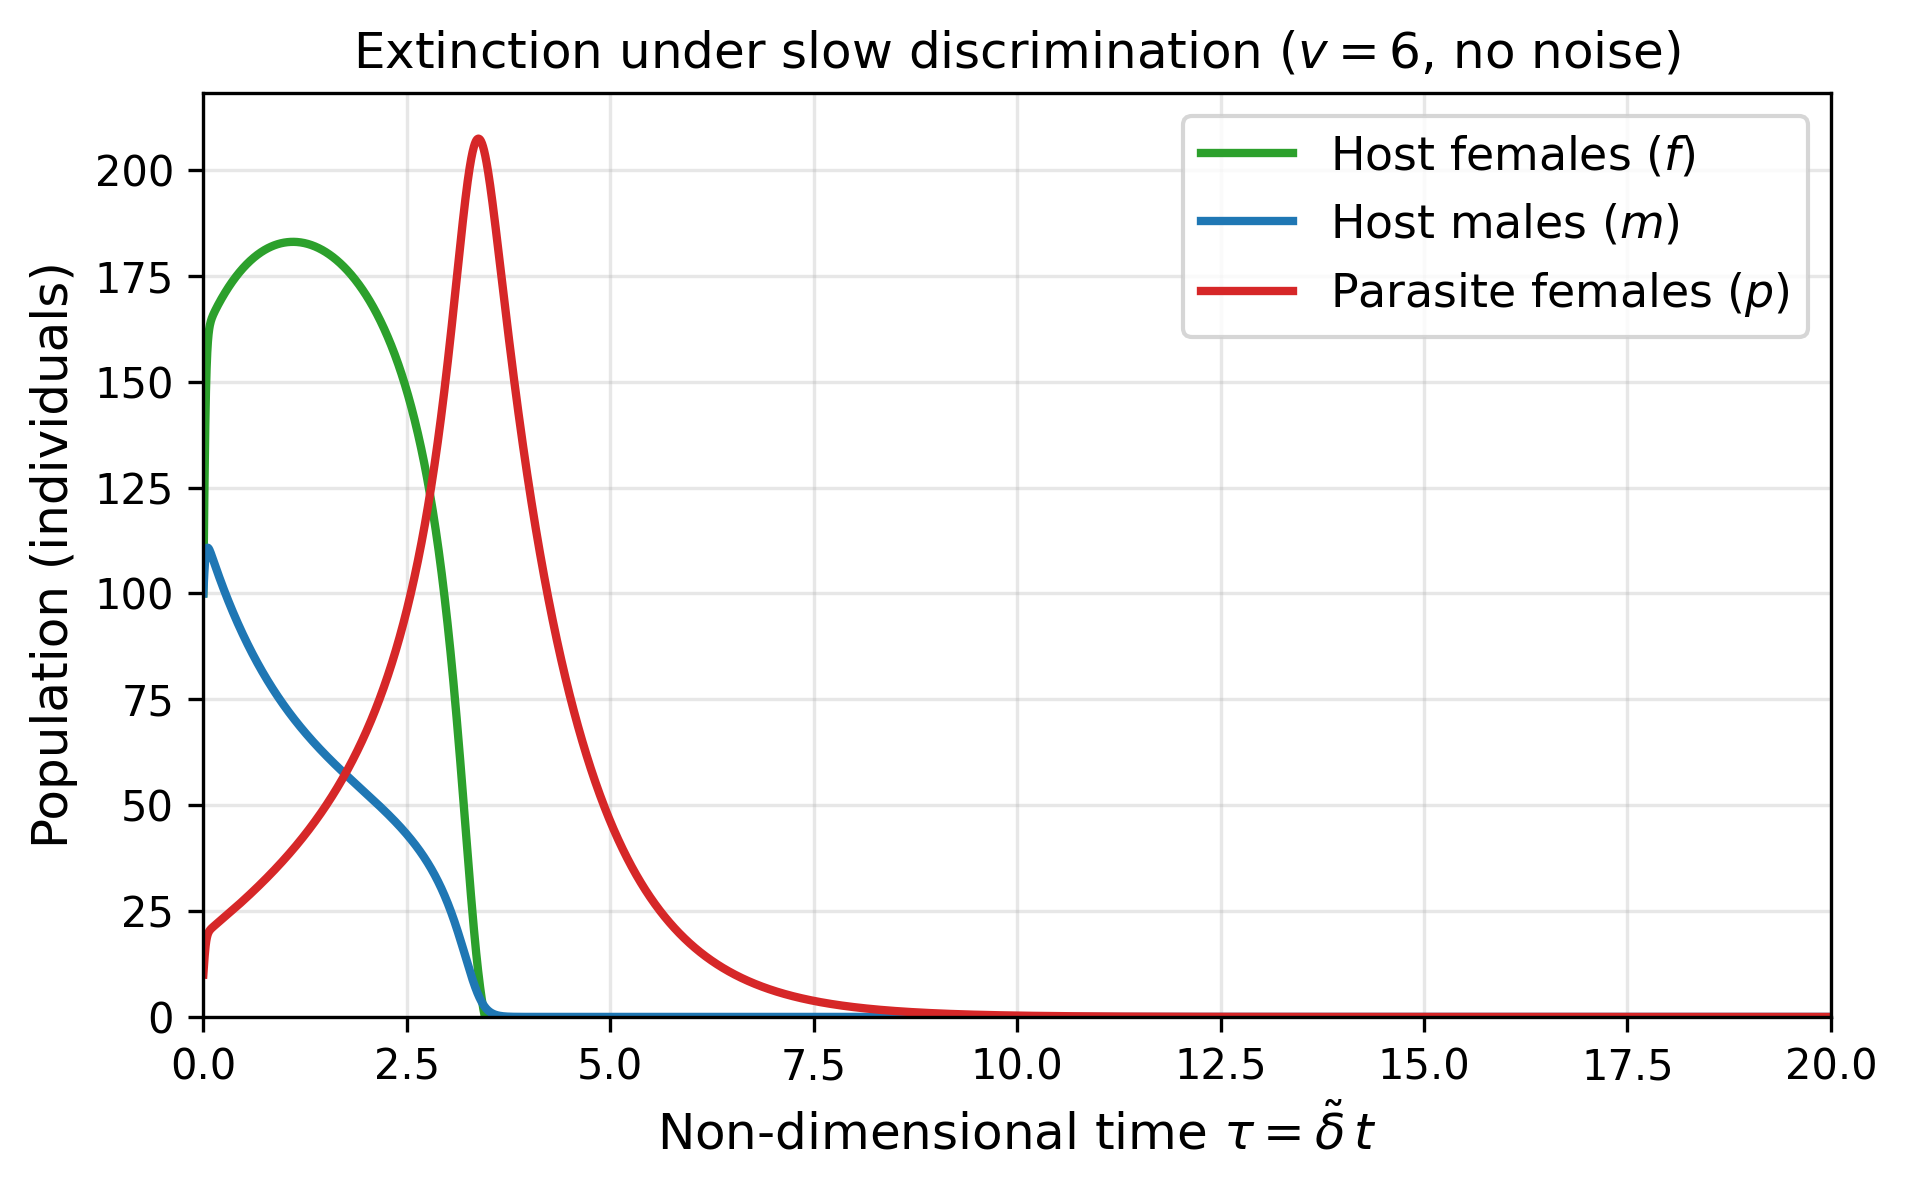
\includegraphics[width=\linewidth]{../poecilia_sde/figures/fig00_extinction_ode.png}
      {\tiny All three populations $\to 0$. No noise, $v=6$, $\tau=20$ ($\approx$200 days).}
    \end{column}
  \end{columns}

\end{frame}

%%-------------------------------------------------
\section{Stochastic Formulations}
\stepcounter{subsection}
%%-------------------------------------------------

%%-------------------------------------------------
%% SLIDE 9: Why Stochasticity?
%%-------------------------------------------------
\begin{frame}{Why Stochasticity?}

  \footnotesize


  \begin{columns}[T]
    \begin{column}{0.55\textwidth}
      \textbf{Environmental evidence:}
      \begin{itemize}
        \item Soto La Marina: seasonal flooding creates alternating isolation and connectivity
        \item During dry season: disconnected pools
        \item During rainy season: pools reconnect
        \item Field data (Balsano 1989): \emph{wide} year-to-year variation in parasite proportion \emph{at the same location}
      \end{itemize}

      \vspace{0.3cm}
      \textbf{Stochastic forcing is not a modeling convenience.\\
      It is a biological fact in this system.}
    \end{column}

    \begin{column}{0.45\textwidth}
      \begin{block}{Three modeling frameworks}
        \textbf{RODE:} piecewise-constant\\
        parametric noise; smooth paths\\[6pt]
        \textbf{It\^{o} SDE:} continuous\\
        multiplicative Wiener noise;\\
        left-endpoint integral\\[6pt]
        \textbf{Stratonovich SDE:} same\\
        noise structure; midpoint\\
        integral; Wong-Zakai limit of\\
        smooth environmental forcing
      \end{block}

      \vspace{0.2cm}
      Each noise structure: \textbf{common}\\
      (shared $W$) or \textbf{independent}\\
      (per-population $W_i$)
    \end{column}
  \end{columns}

\end{frame}

%%-------------------------------------------------
%% SLIDE 10: Five Formulations Overview
%%-------------------------------------------------
\begin{frame}{Five Formulations — One Biological System}

    \footnotesize


  \begin{center}
  \renewcommand{\arraystretch}{1.1}
  \begin{tabular}{llll}
    \toprule
    \textbf{\#} & \textbf{Formulation} & \textbf{Noise} & \textbf{Biological interpretation} \\
    \midrule
    1 & RODE & Piecewise-constant & Discrete environmental pulses \\
    2 & It\^{o} / common & Single $W(t)$ & Shared habitat driver \\
    3 & It\^{o} / independent & $W_f, W_m, W_p$ & Independent fluctuations \\
    4 & Stratonovich / common & Single $W(t)$ & Limit of smooth forcing \\
    5 & Stratonovich / indep. & $W_f, W_m, W_p$ & Limit of smooth, independent \\
    \bottomrule
  \end{tabular}
  \end{center}

  \vspace{0.3cm}
  \begin{alertblock}{The central question of this talk}
    These are not five ways to write the same model.\\
    They encode \textbf{different physical assumptions} and produce\\
    \textbf{different quantitative predictions} for extinction probability.\\[4pt]
    A researcher who picks one and reports it as ``the stochastic model''\\
    is presenting \textbf{one answer among five}.
  \end{alertblock}

\end{frame}

%%-------------------------------------------------
%% SLIDE 11: RODE Formulation
%%-------------------------------------------------
\begin{frame}{RODE: Random Ordinary Differential Equation}

    \footnotesize

    \begin{columns}[T]
    \begin{column}{0.52\textwidth}
      Noise enters as piecewise-constant perturbation to death rate:
      \[
        \frac{df}{d\tau} = a\beta L m(f-\gamma p) - (1-\eta_f)f
      \]
      $\eta_i(t) \sim \mathrm{Uniform}[0, \tilde{\eta}_{\max}]$,
      resampled each step.

      \vspace{0.2cm}
      \textbf{Key property:} between resampling events, system is a
      standard ODE $\Rightarrow$ classical RK45 applies.

      \vspace{0.3cm}
      \textbf{Noise structure} (from Balsano 1989 association data):
      \[
        \eta_f = \eta_m = \tfrac{2}{3}\eta, \quad \eta_p = \eta
      \]
      Parasite females bear full environmental load; host populations
      bear two-thirds.
    \end{column}

    \begin{column}{0.48\textwidth}
      \begin{block}{RODE Boundary Dissipativity Lemma}
        On the population ceiling $f+m+p=1$:\\[4pt]
        $\nabla\cdot\mathbf{F}\big|_{f+m+p=1}
          \leq \eta_f + \eta_m + \eta_p - 3$\\[6pt]
        System is \textbf{dissipative} at the ceiling whenever:
        \[
          \eta_f + \eta_m + \eta_p < 3
        \]
        i.e., noise amplitudes sum below the death rate threshold.
      \end{block}

      \vspace{0.2cm}
      \textit{Proof:} At $L=0$, all birth terms vanish.\\
      Liouville's theorem gives phase-space\\
      contraction directly.
    \end{column}
  \end{columns}

\end{frame}

%%-------------------------------------------------
%% SLIDE 12: Itô SDE Formulation
%%-------------------------------------------------
\begin{frame}{It\^{o} SDE: Multiplicative Geometric Noise}

    \footnotesize

    \textbf{Common noise} (single Wiener process $W$):
  \[
    df = \mu_f(\mathbf{u})\,dt + \sigma_f f\,dW, \quad
    dm = \mu_m(\mathbf{u})\,dt + \sigma_m m\,dW, \quad
    dp = \mu_p(\mathbf{u})\,dt + \sigma_p p\,dW
  \]

  \vspace{0.2cm}
  \textbf{Key analytical result — mean equations (Proposition 1):}

  \begin{block}{It\^{o} noise does NOT shift ensemble means}
    Under mean-field closure, $F = \E[f]$, $M = \E[m]$, $P = \E[p]$ satisfy
    \emph{exactly the deterministic ODE}.\\[4pt]
    Proof: the stochastic integral $\int \sigma_f f\,dW$ is a martingale;
    $\E[\Delta W \mid \mathcal{F}_t] = 0$ eliminates the noise term.
  \end{block}

  \vspace{0.3cm}
  \textbf{Scalar Lyapunov exponent} for parasite $p$-subsystem:
  \[
    \lambda_{\text{It\^{o}}} = \beta_{\text{eff}} - \delta - \half\sigma_p^2
  \]
  Extinction ($\lambda < 0$) requires $\sigma_p > \sqrt{2(\beta_{\text{eff}}-\delta)}$.\\
  \textbf{Increasing It\^{o} noise promotes extinction of the parasite.}

\end{frame}

%%-------------------------------------------------
%% SLIDE 13a: Stratonovich and Wong-Zakai — Plain Terms
%%-------------------------------------------------
\begin{frame}{Stratonovich and Wong-Zakai: What Do They Mean?}
  \tiny

  \begin{columns}[T]

    \begin{column}{0.48\textwidth}
      \begin{block}{The It\^{o} vs.\ Stratonovich question}
        Both write $dX = \mu\,dt + \sigma X\,dW$.\\[6pt]
        They differ in \textbf{when} the integrand\\
        is evaluated inside $\int g(X)\,dW$:
        \begin{itemize}
          \item \textbf{It\^{o}:} left endpoint of each interval\\
                $\Rightarrow$ integrand evaluated \emph{before} the noise kick
          \item \textbf{Stratonovich:} midpoint\\
                $\Rightarrow$ integrand evaluated \emph{during} the noise kick
        \end{itemize}
        \vspace{0.2cm}
        For \textbf{additive} noise: identical.\\
        For \textbf{multiplicative} noise ($g = \sigma X$):\\
        the midpoint rule adds an extra drift term $+\half\sigma^2 X$.\\[4pt]
        \textcolor{alertred}{Same equation. Different calculus. Different physics.}
      \end{block}
    \end{column}

    \begin{column}{0.52\textwidth}
      \begin{block}{The Wong-Zakai theorem in plain language}
        \textbf{Question:} Real environmental noise is never
        truly white. It is \emph{colored} --- it has a
        finite correlation time $\tau_c$ (e.g., a flood
        lasts days, not an instant).\\[6pt]
        \textbf{What happens as $\tau_c \to 0$?}\\[4pt]
        Replace white noise $W(t)$ with a smooth
        approximation $W^\epsilon(t)$ with correlation
        time $\epsilon$, solve the ODE, then take
        $\epsilon \to 0$.\\[6pt]
        \textbf{Wong \& Zakai (1965):} the limit is the
        \textbf{Stratonovich} SDE, not the It\^{o} SDE.\\[6pt]
        \textbf{Plain conclusion:} if your noise is a
        physical process smoothed over a short time
        scale --- seasonal flooding, temperature
        oscillations, pool connectivity ---
        \textcolor{alertred}{\textbf{Stratonovich is the
        correct limit, not a convention.}}
      \end{block}
    \end{column}

  \end{columns}

  \begin{center}
    \footnotesize
    For \textit{P.~formosa}: Soto La Marina flooding has correlation
    time $\sim$ weeks to months $\Rightarrow$ Stratonovich is
    physically motivated, It\^{o} is a mathematical convenience.
  \end{center}

\end{frame}

%%-------------------------------------------------
%% SLIDE 13: Stratonovich SDE Formulation
%%-------------------------------------------------
\begin{frame}{Stratonovich SDE: The Wong-Zakai Limit}

  \footnotesize

  \textbf{Stratonovich formulation} (midpoint integral):
  \[
    df = \mu_f\,dt + \sigma_f f \circ dW
  \]

  It\^{o}--Stratonovich conversion adds drift correction
  $+\half\sigma_i^2 u_i$ per population.

  \vspace{0.2cm}
  \begin{block}{Stratonovich noise DOES shift ensemble means (Proposition 2)}
    \[
      \frac{dF}{dt} = a\beta(1-F-M-P)M(F-\gamma P) - \delta F
      + \textcolor{alertred}{\half\sigma_f^2 F}
    \]
    The noise-induced increment $+\half\sigma_i^2 u_i$ acts as an
    \textbf{effective noise-induced birth rate}. Since $\sigma_p > \sigma_f = \sigma_m$ (parasite bears more noise),
    the parasite receives the \textbf{largest growth bonus}.
  \end{block}

  \vspace{0.2cm}
  \textbf{Scalar Lyapunov exponent:}
  \[
    \lambda_{\text{Strat}} = \beta_{\text{eff}} - \delta
    \quad \textbf{(independent of } \sigma_p \textbf{!)}
  \]
  The Stratonovich correction $+\half\sigma_p^2$ in the drift is exactly
  cancelled by the It\^{o} correction $-\half\sigma_p^2$ in $d\ln p$.\\
  \textcolor{alertred}{\textbf{No amount of Stratonovich noise stabilizes the system by suppressing parasite growth.}}

\end{frame}

%%-------------------------------------------------
\section{Results}
\stepcounter{subsection}
%%-------------------------------------------------

%%-------------------------------------------------
%% SLIDE 14: Single Trajectory Comparison
%%-------------------------------------------------
\begin{frame}{Single Trajectory: All Five Formulations}
  \footnotesize

  \begin{center}
    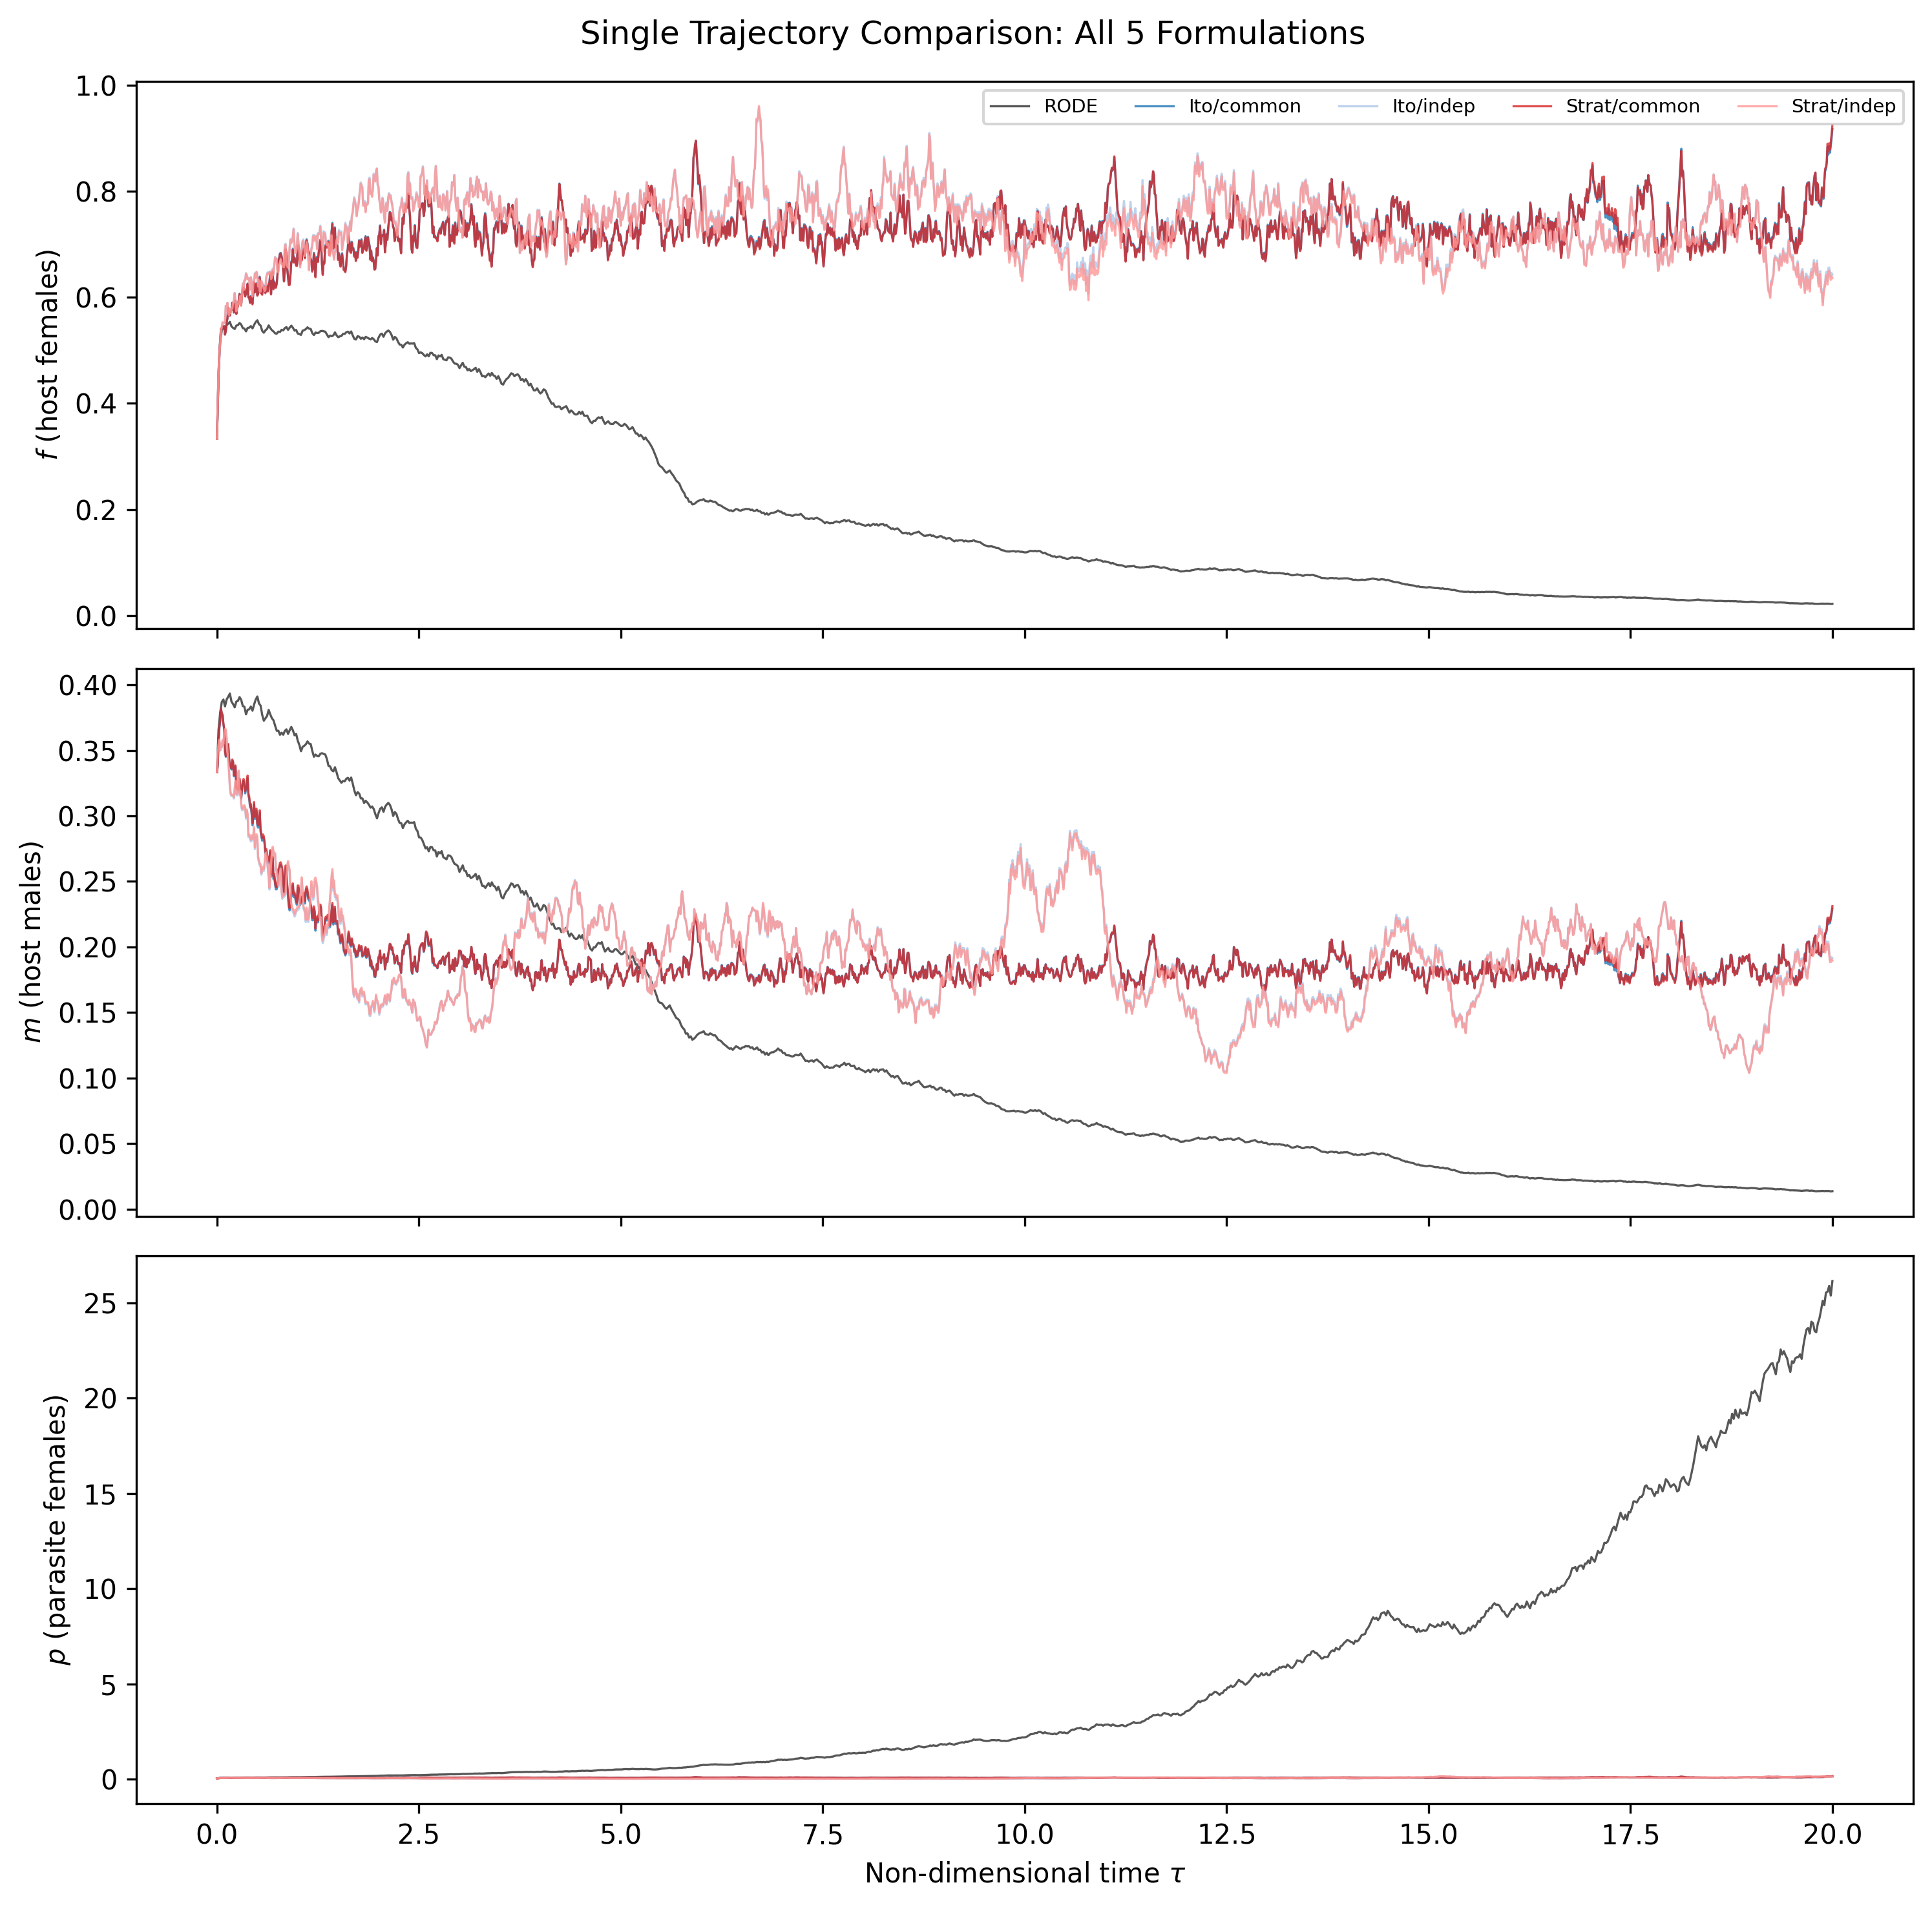
\includegraphics[width=0.6\textwidth]{../poecilia_sde/figures/fig05_single_trajectory_comparison.png}
  \end{center}
  {\footnotesize
  Slow discrimination ($v=6$): extinction in all formulations.
  Fast discrimination ($v=60$): coexistence in all formulations.
  The \emph{qualitative} outcome is robust; quantitative trajectories differ.}

\end{frame}

%%-------------------------------------------------
%% SLIDE 15: Ensemble Statistics
%%-------------------------------------------------
\begin{frame}{Ensemble Statistics: Mean $\pm$ 95\% CI, $n=500$ Paths}

    \footnotesize
  \begin{center}
    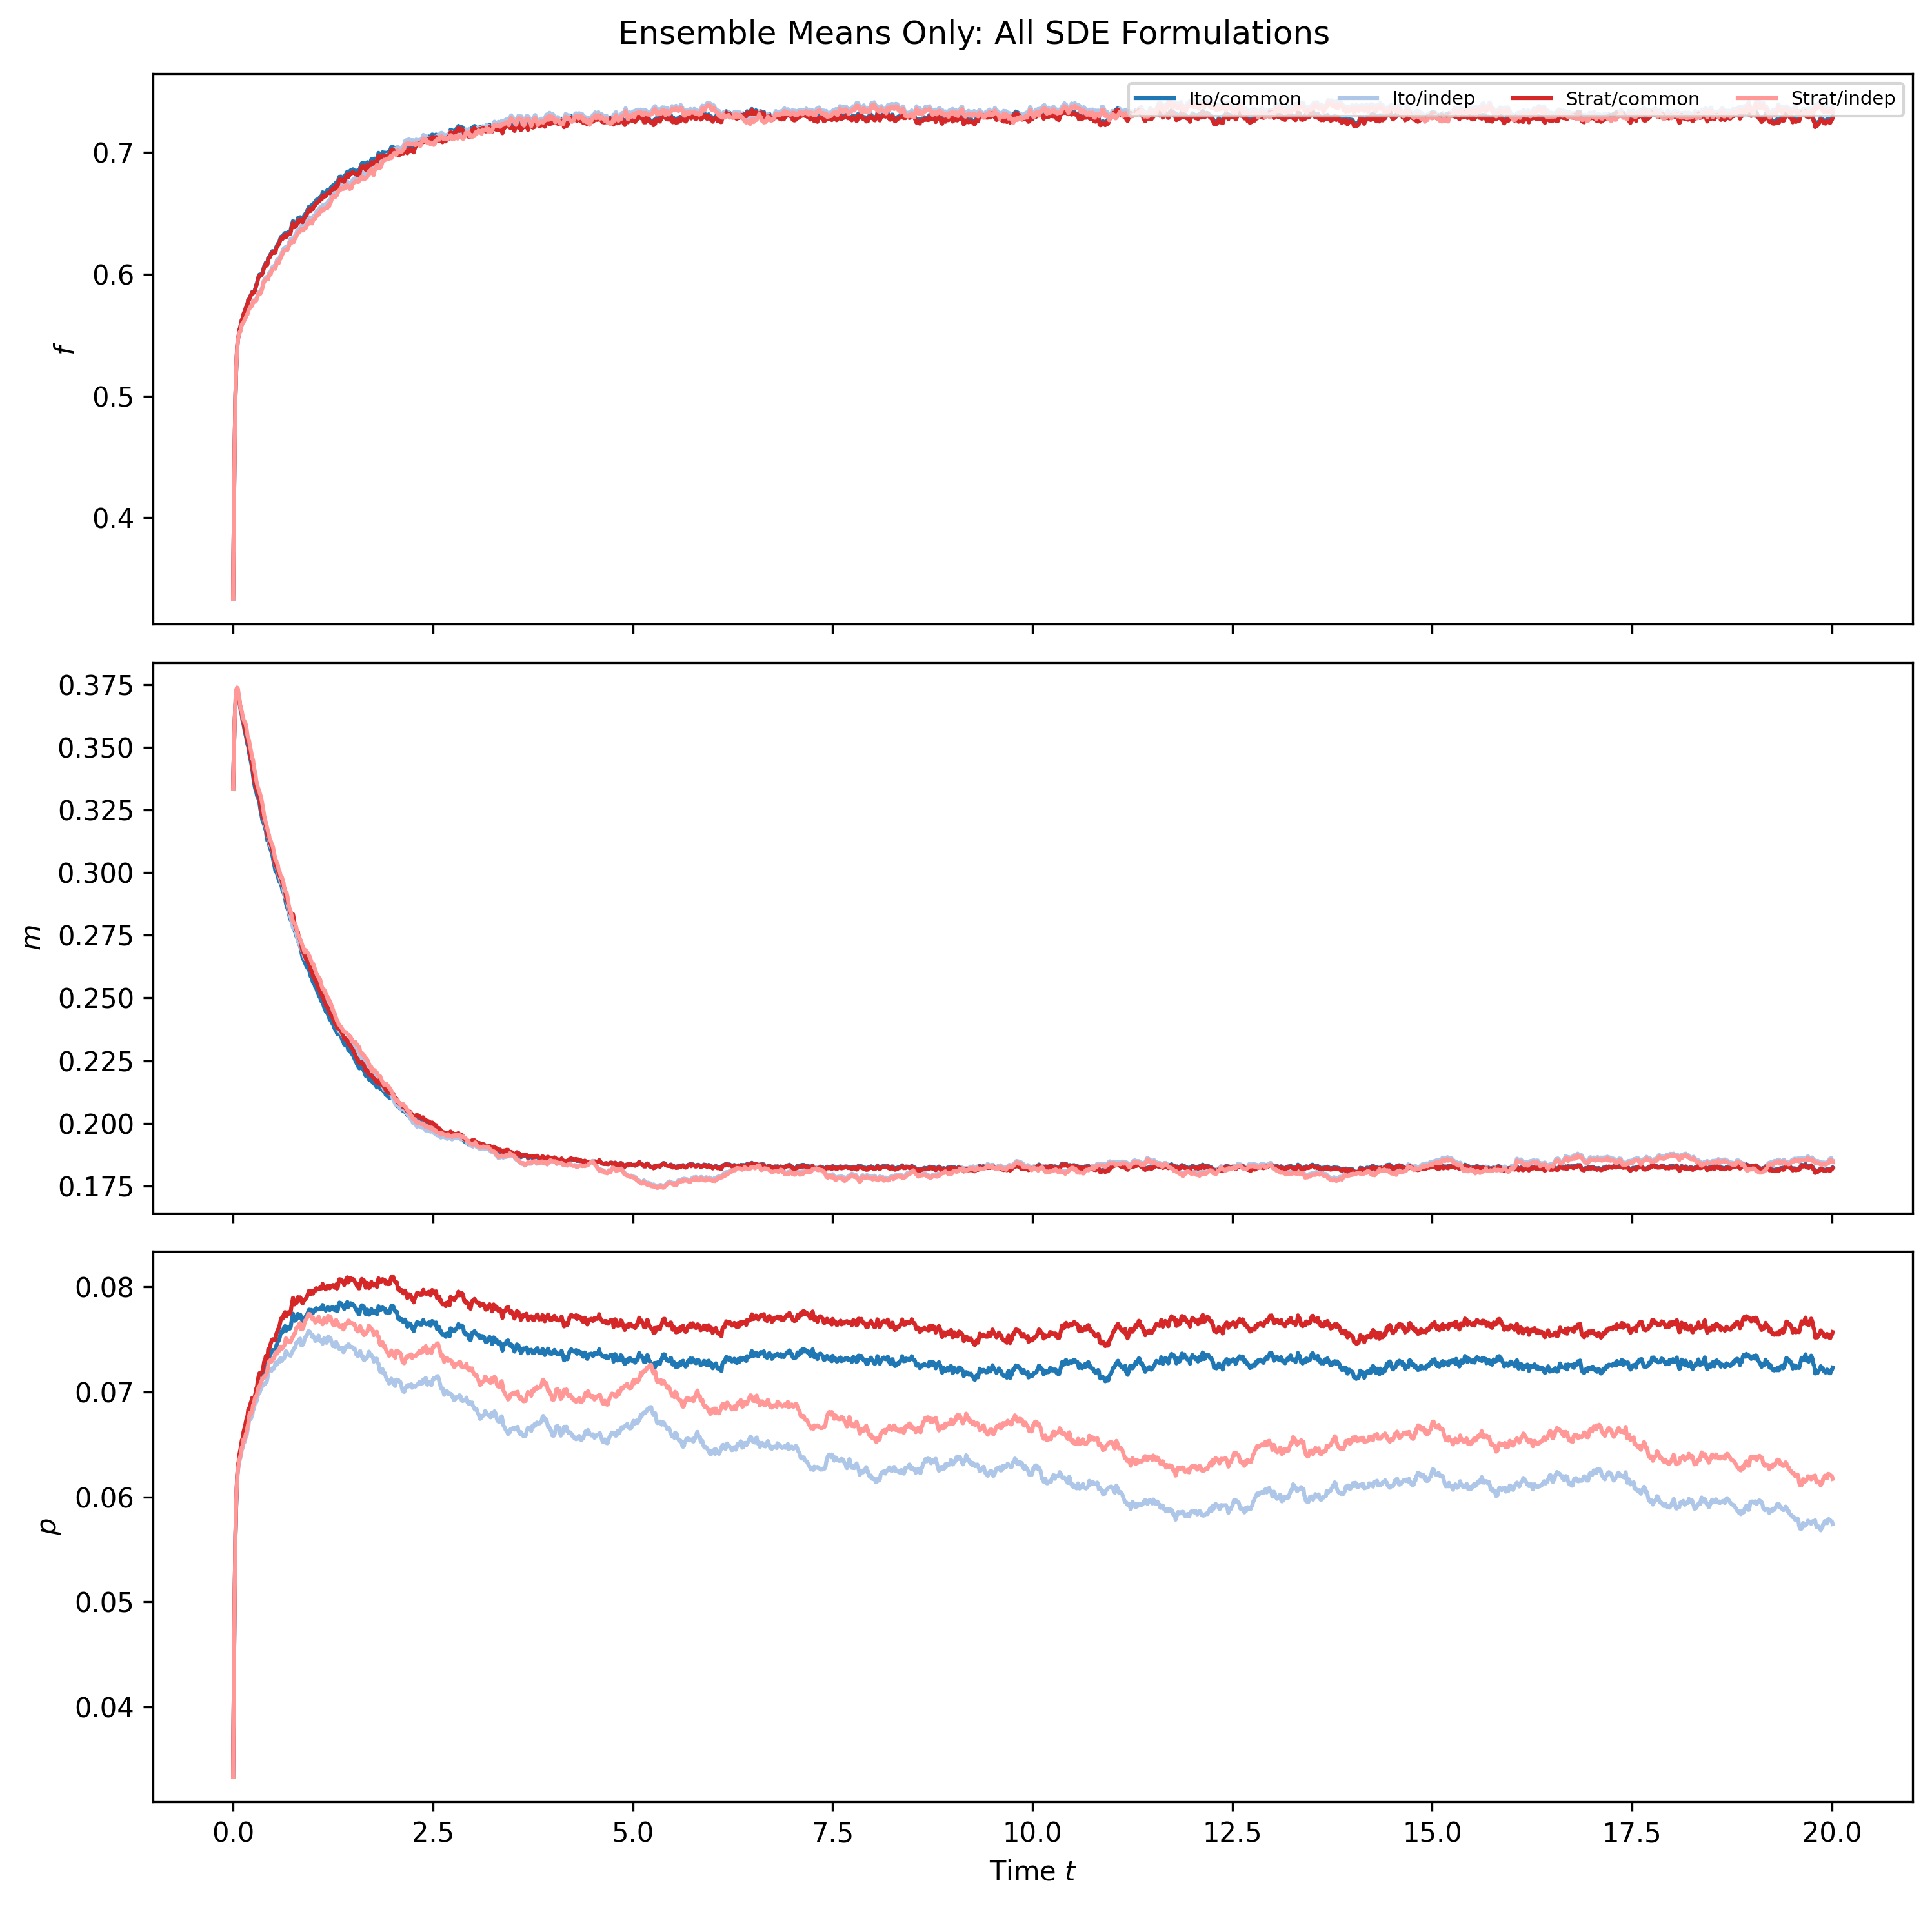
\includegraphics[width=0.6\textwidth]{../poecilia_sde/figures/fig06_ensemble_means_only.png}
  \end{center}
  {\footnotesize
  Stratonovich (red) sits systematically above It\^{o} (blue) --- the
  noise-induced mean shift predicted by Proposition~2.
  RODE (dark) differs in mean level due to positive mean noise bias
  ($\E[\eta] = \tilde\eta_{\max}/2 > 0$).}

\end{frame}


%%-------------------------------------------------
%% SLIDE 16a: Moment Closure — Plain Explanation
%%-------------------------------------------------
\begin{frame}{Moment Closure: What Is It and Why Do We Need It?}
  \tiny

  \begin{columns}[T]

    \begin{column}{0.48\textwidth}
      \begin{block}{The moment hierarchy problem}
        Take expectations of the SDE for $f$:
        \[
          \frac{d\E[f]}{dt} = \E\bigl[a\beta(1-f-m-p)\,m\,(f-\gamma p)\bigr]
        \]
        The right side contains $\E[fm]$, $\E[mp]$, $\E[fmp]$, \ldots\\[6pt]
        To find $\E[fm]$ we need $\E[f^2m]$.\\
        To find $\E[f^2m]$ we need $\E[f^3m]$.\\[6pt]
        \textcolor{alertred}{\textbf{The hierarchy never closes.}}\\[4pt]
        An exact ODE for means requires\\
        knowing all higher moments.
      \end{block}
    \end{column}

    \begin{column}{0.52\textwidth}
      \begin{block}{Mean-field closure: the approximation}
        \textbf{Assumption:} populations fluctuate\\
        nearly independently near the mean, so:
        \[
          \E[f \cdot m] \approx \E[f]\cdot\E[m] = F \cdot M
        \]
        Replace all products inside expectations\\
        with products of means.\\[6pt]
        \textbf{Result:} the infinite hierarchy collapses\\
        to a \emph{finite} ODE system in $(F, M, P)$.\\[6pt]
        \textbf{Exact when:} $f$ and $m$ are uncorrelated.\\
        \textbf{Approximate when:} correlations are weak\\
        relative to the mean trajectory.
      \end{block}

      \vspace{0.2cm}
      \begin{block}{What it gives us}
        \begin{itemize}
          \item Analytical mean trajectories without Monte Carlo
          \item Explicit formula for noise-induced mean shift (Stratonovich)
          \item Validated against $n=500$ path ensembles (previous slide)
        \end{itemize}
      \end{block}
    \end{column}

  \end{columns}

\end{frame}

%%-------------------------------------------------
%% SLIDE 16: Moment Equations vs Monte Carlo
%%-------------------------------------------------
\begin{frame}{Moment Closure Validation}

  \begin{columns}[T]
    \begin{column}{0.5\textwidth}
      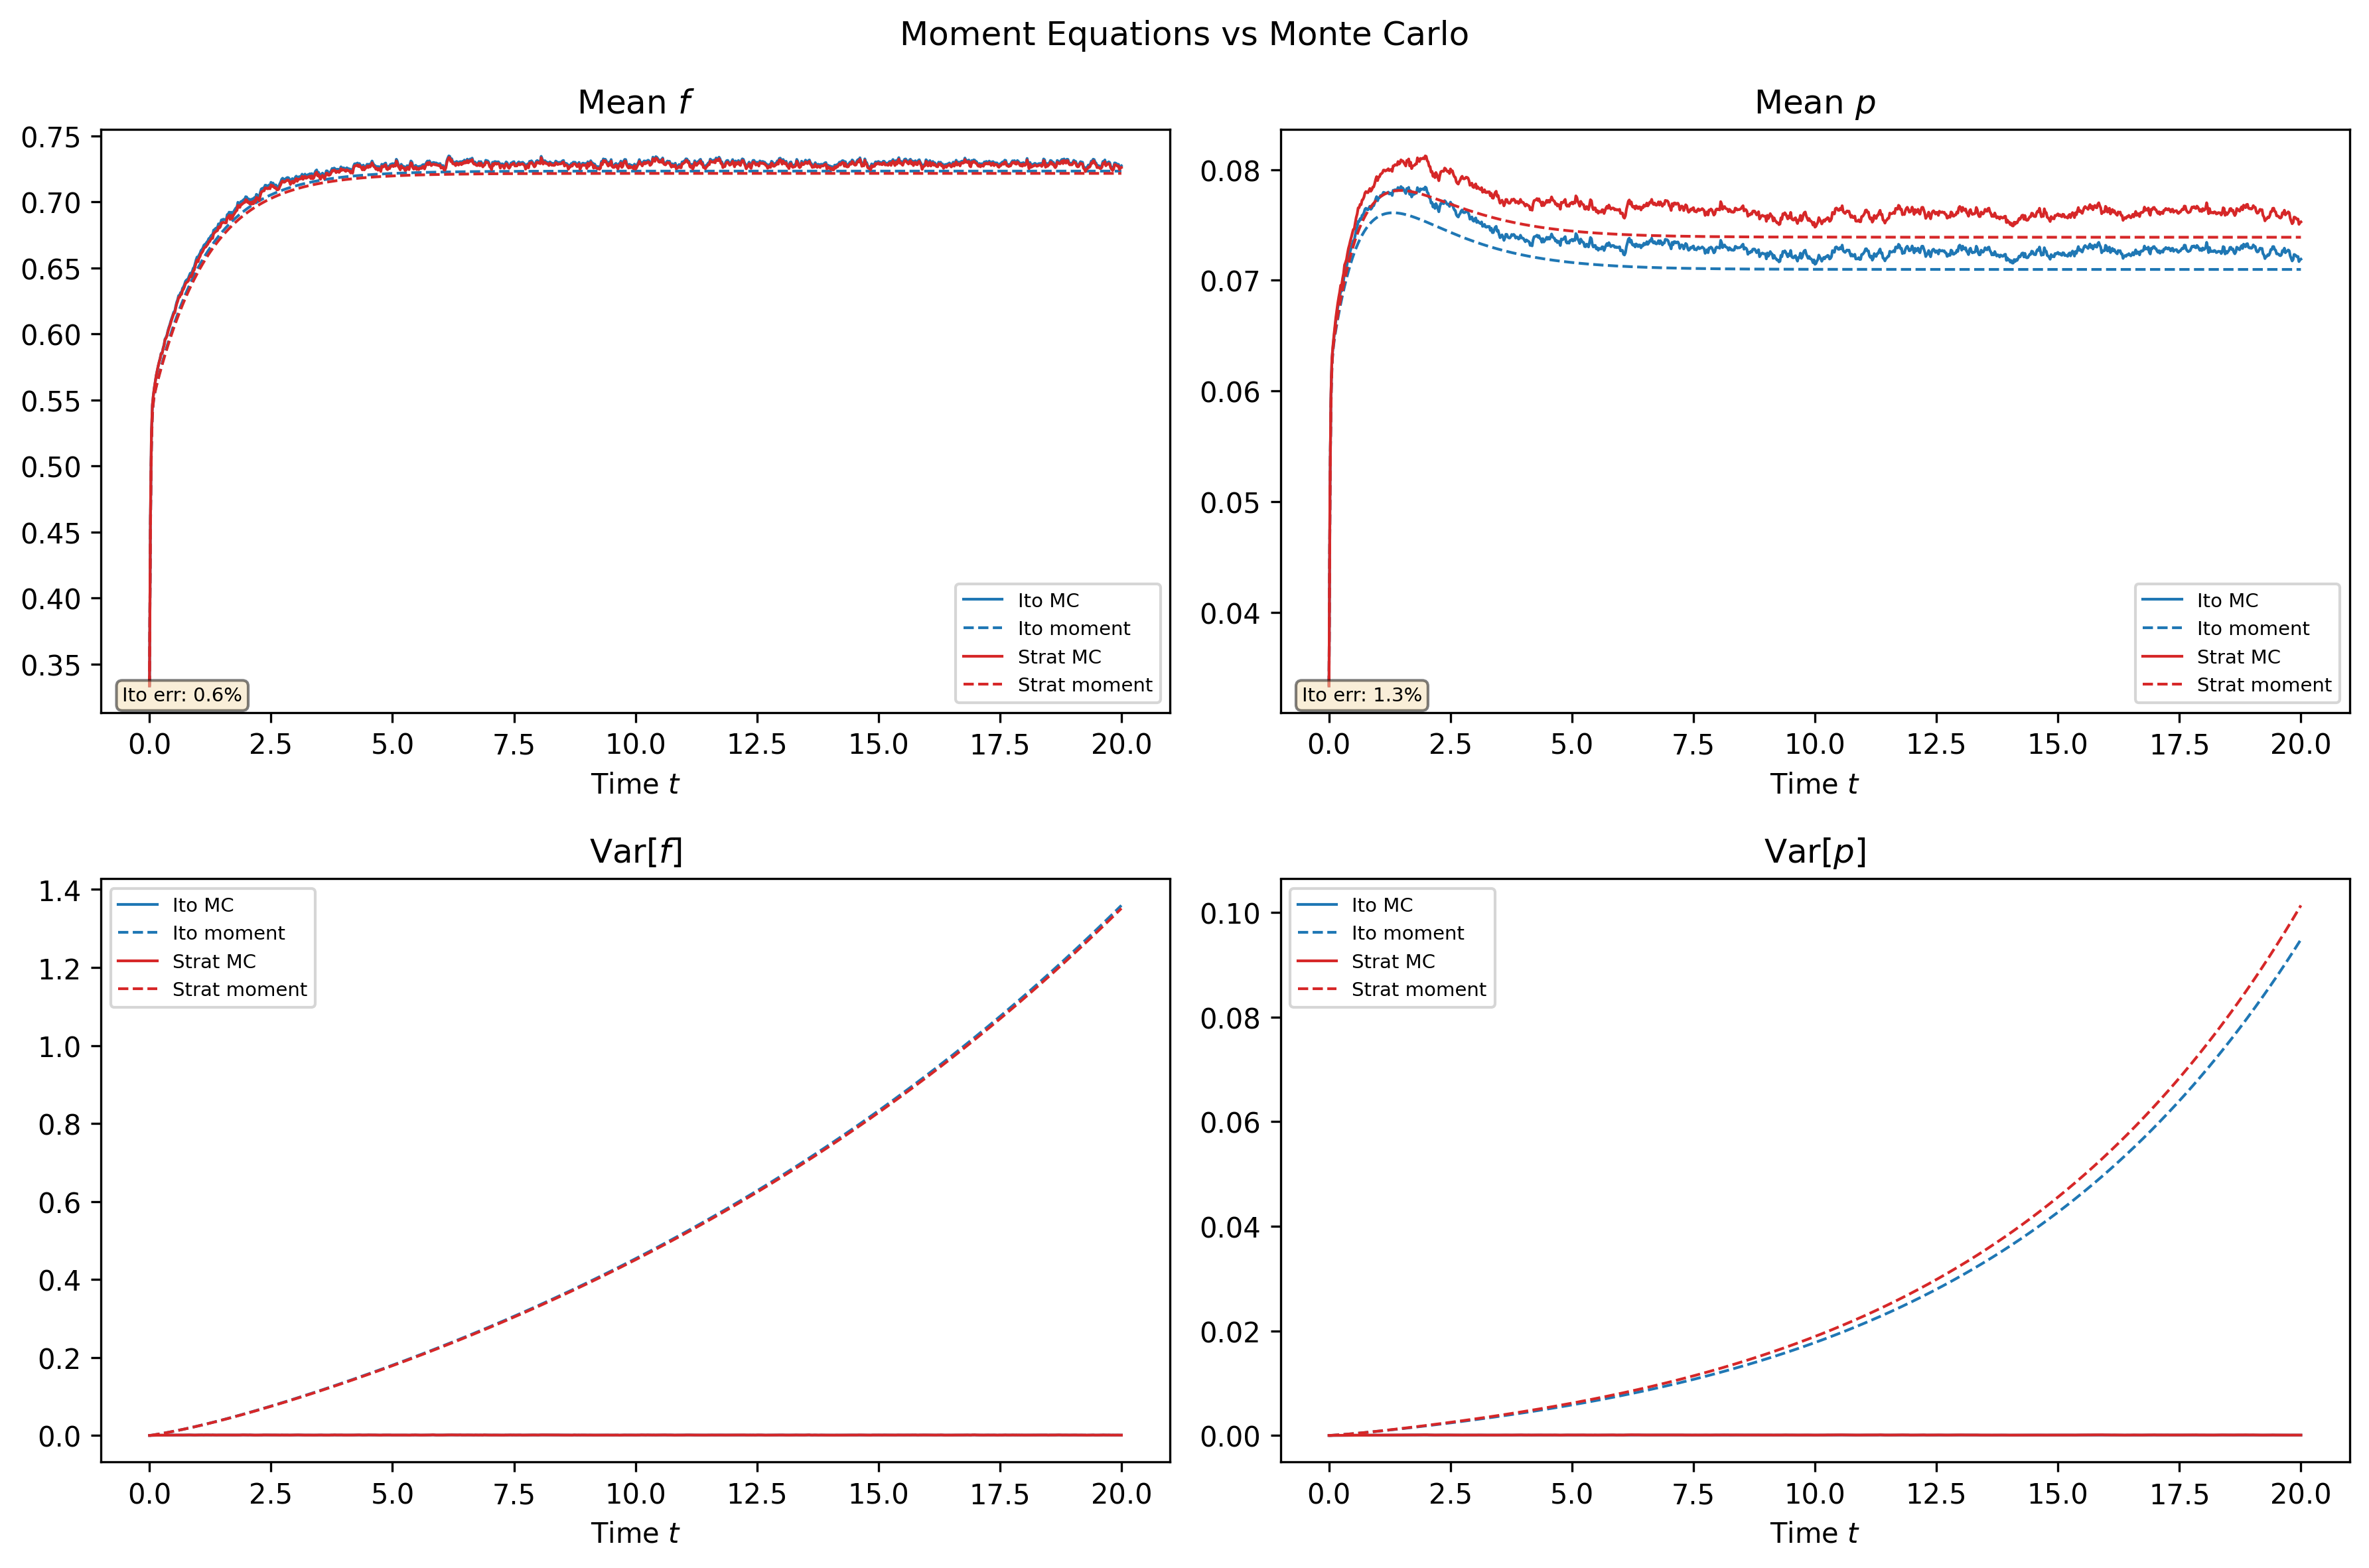
\includegraphics[width=\linewidth]{../poecilia_sde/figures/fig07_moment_vs_montecarlo.png}
    \end{column}
    \begin{column}{0.5\textwidth}
      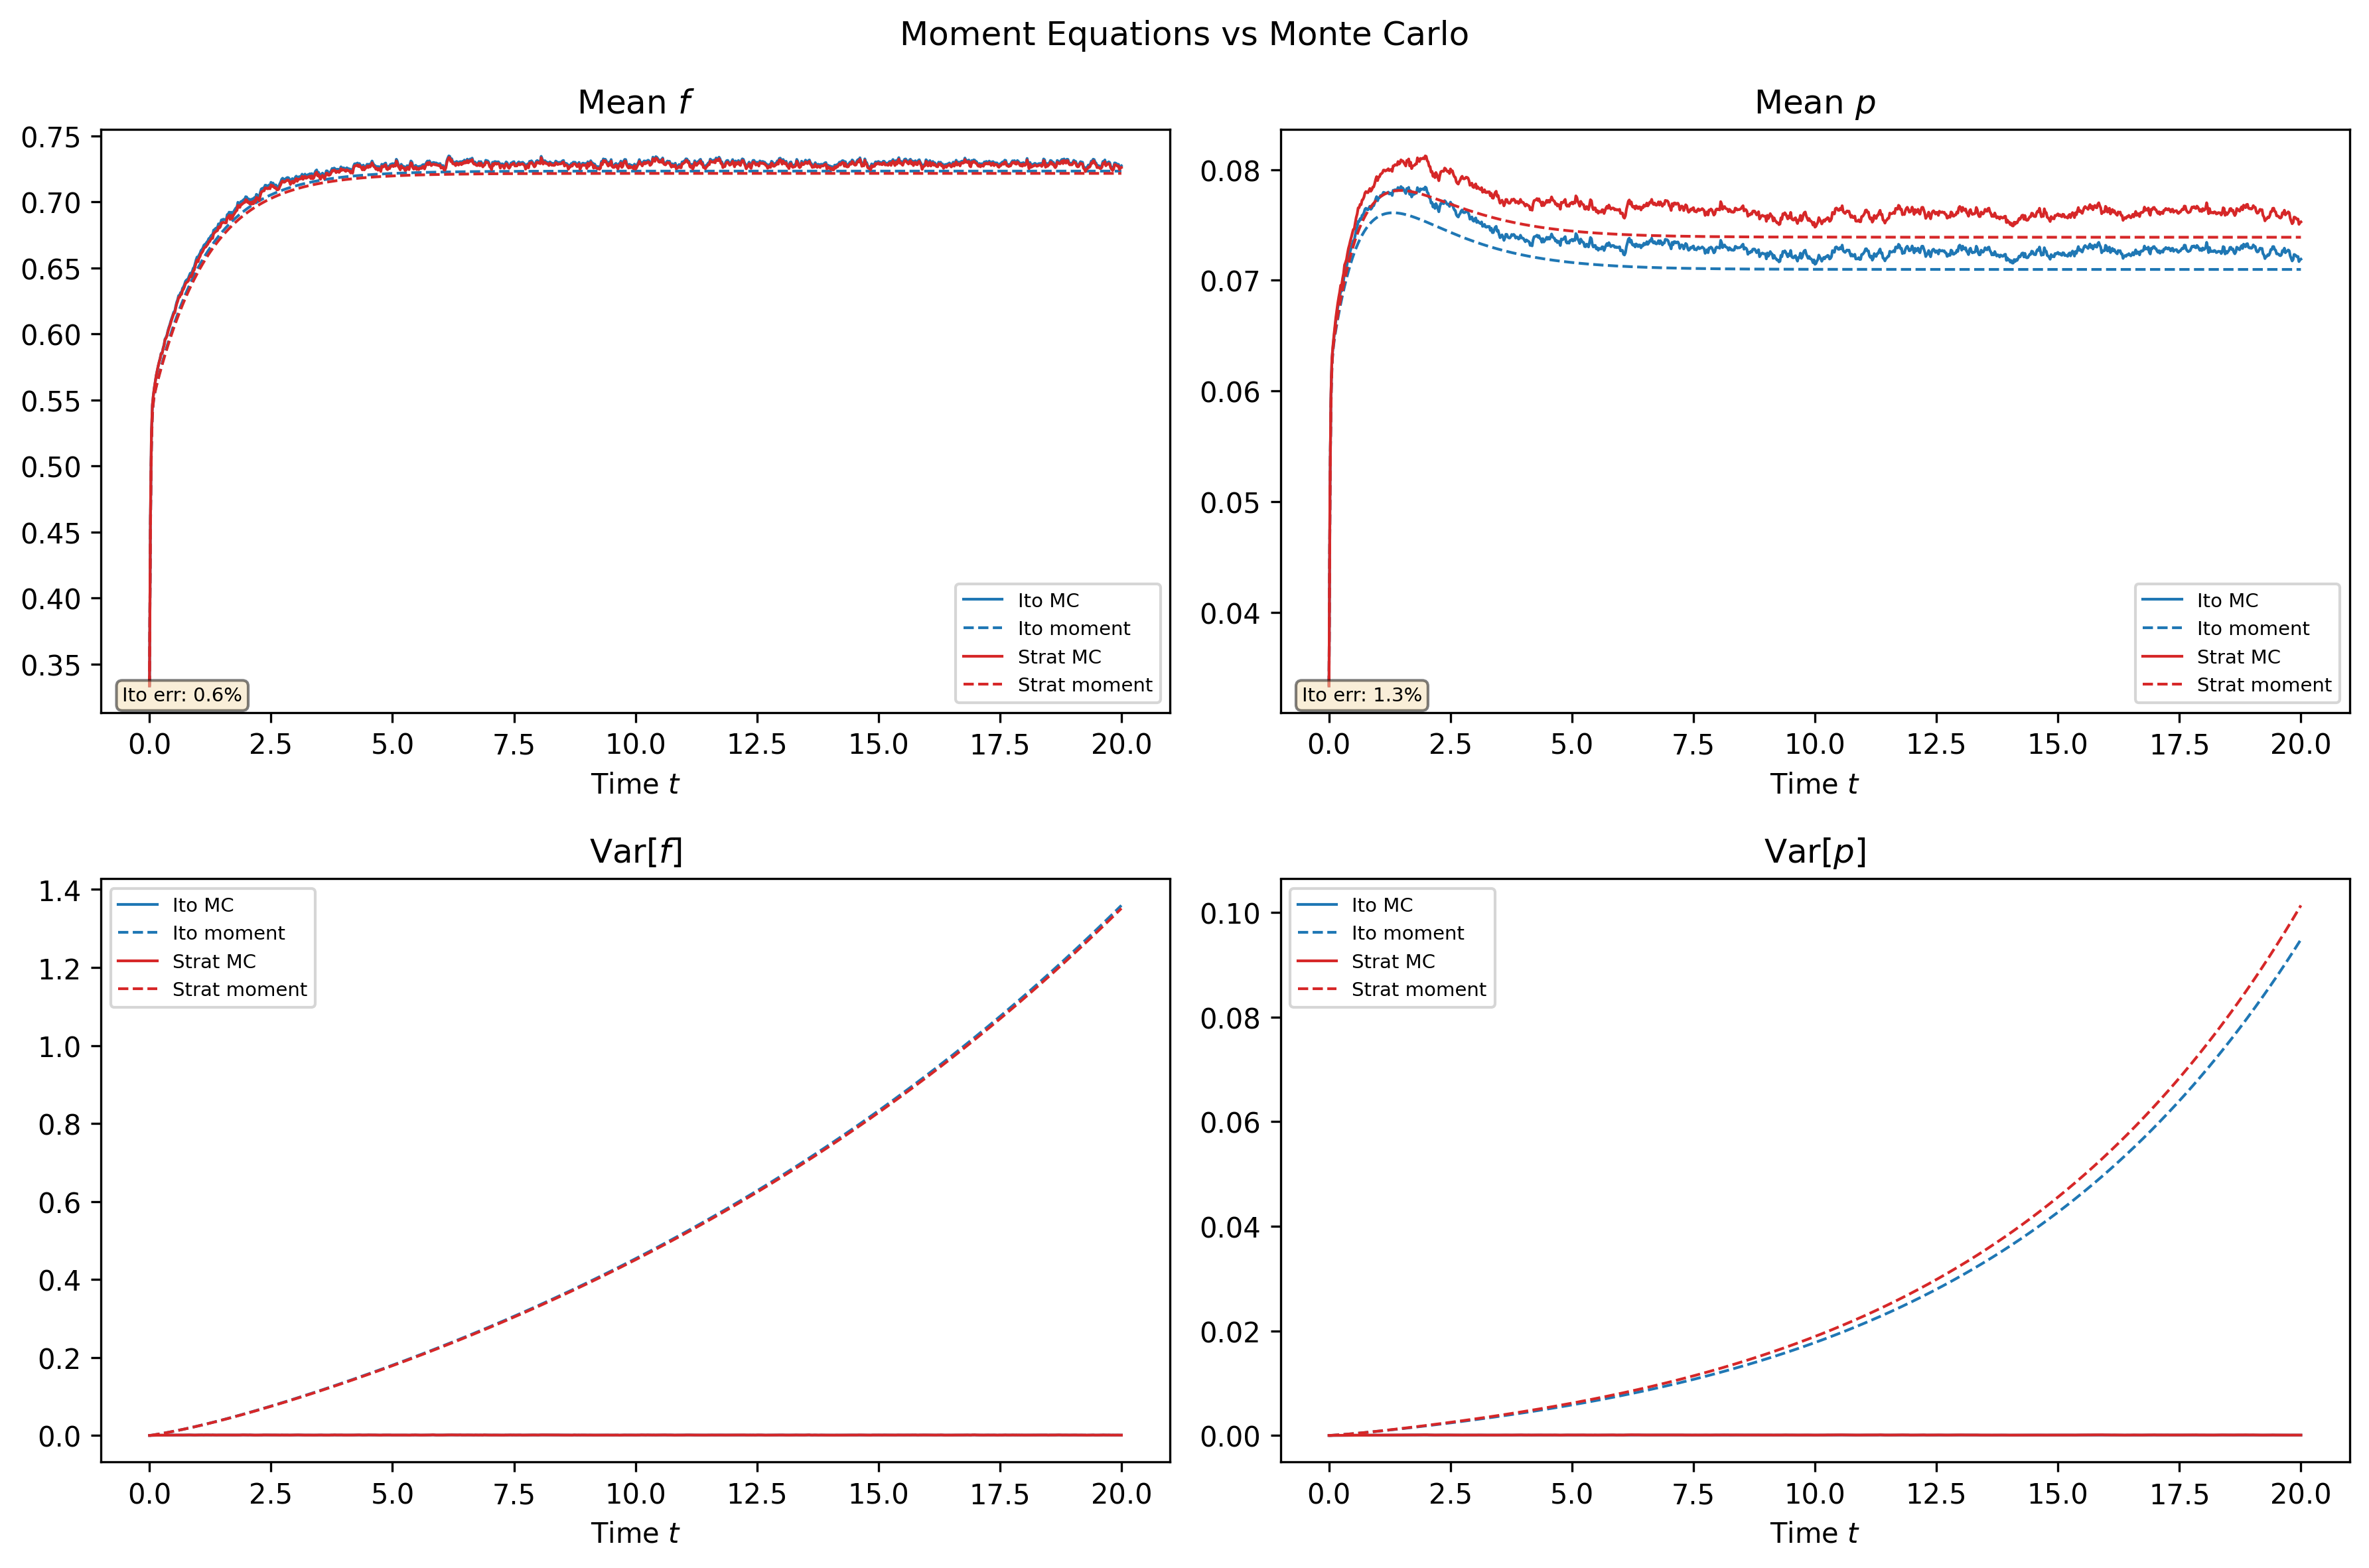
\includegraphics[width=\linewidth]{../poecilia_sde/figures/fig08_moment_vs_montecarlo.png}
    \end{column}
  \end{columns}

  {\footnotesize
  Dashed lines: moment equations under mean-field closure.
  Solid lines: Monte Carlo ensemble means ($n=500$).
  \textbf{Left:} It\^{o}/common noise --- moment closure tracks MC well.
  \textbf{Right:} Stratonovich/common noise --- upward shift confirmed analytically and numerically.}

\end{frame}

%%-------------------------------------------------
%% SLIDE 18: Noise Structure Sensitivity
%%-------------------------------------------------
\begin{frame}{Noise Structure Sensitivity: Common vs.\ Independent}
  \footnotesize

  \begin{center}
    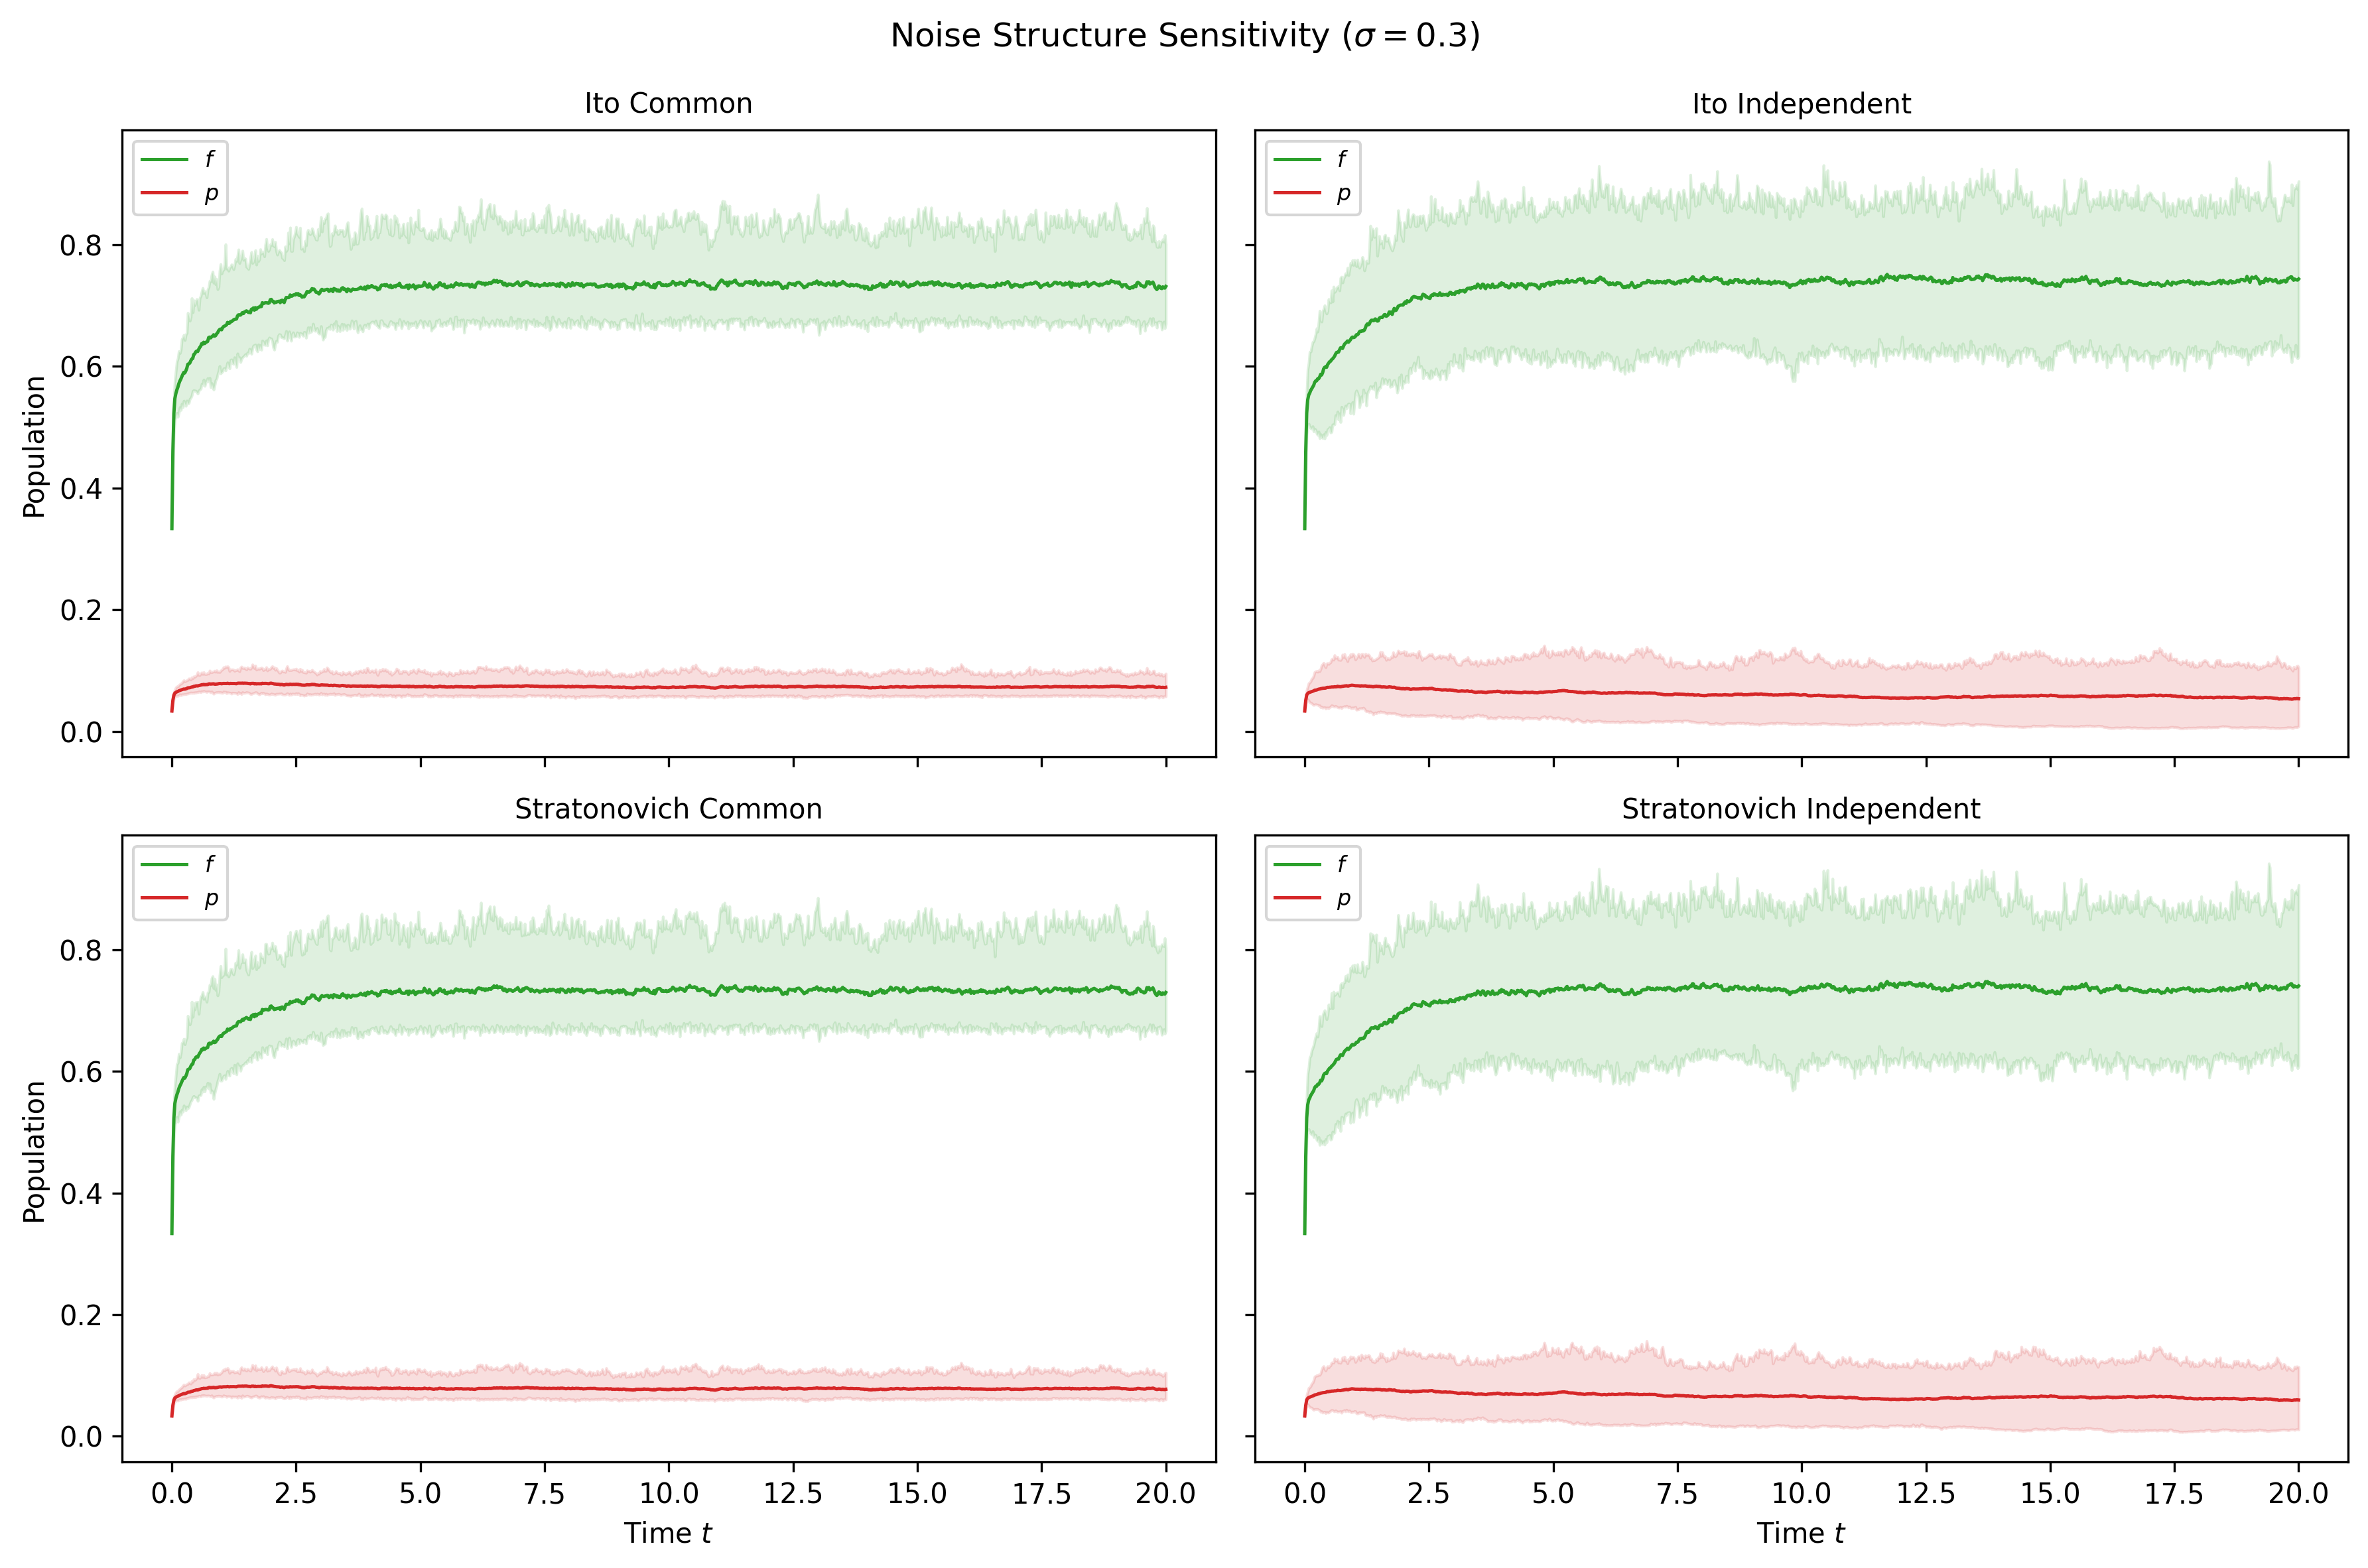
\includegraphics[width=0.85\textwidth]{../poecilia_sde/figures/fig09_noise_structure_sensitivity.png}
  \end{center}

  {\footnotesize
  \textbf{Common noise:} covariance driven by $\sigma_f\sigma_m(FM + \mathrm{Cov}(f,m))$ ---
  populations fluctuate coherently; cross-driving can reduce effective competition when $p>f$.\\
  \textbf{Independent noise:} cross-driving term vanishes at mean-field level;
  deterministic coupling still generates covariance through shared nonlinear drift.\\
  Noise \emph{architecture} matters, not just noise amplitude.}

\end{frame}



%%-------------------------------------------------
%% SLIDE 17: Stability Boundaries
%%-------------------------------------------------
\begin{frame}{Stability Boundaries: All Five Formulations}

  \footnotesize
  \begin{columns}[T]
    \begin{column}{0.60\textwidth}
      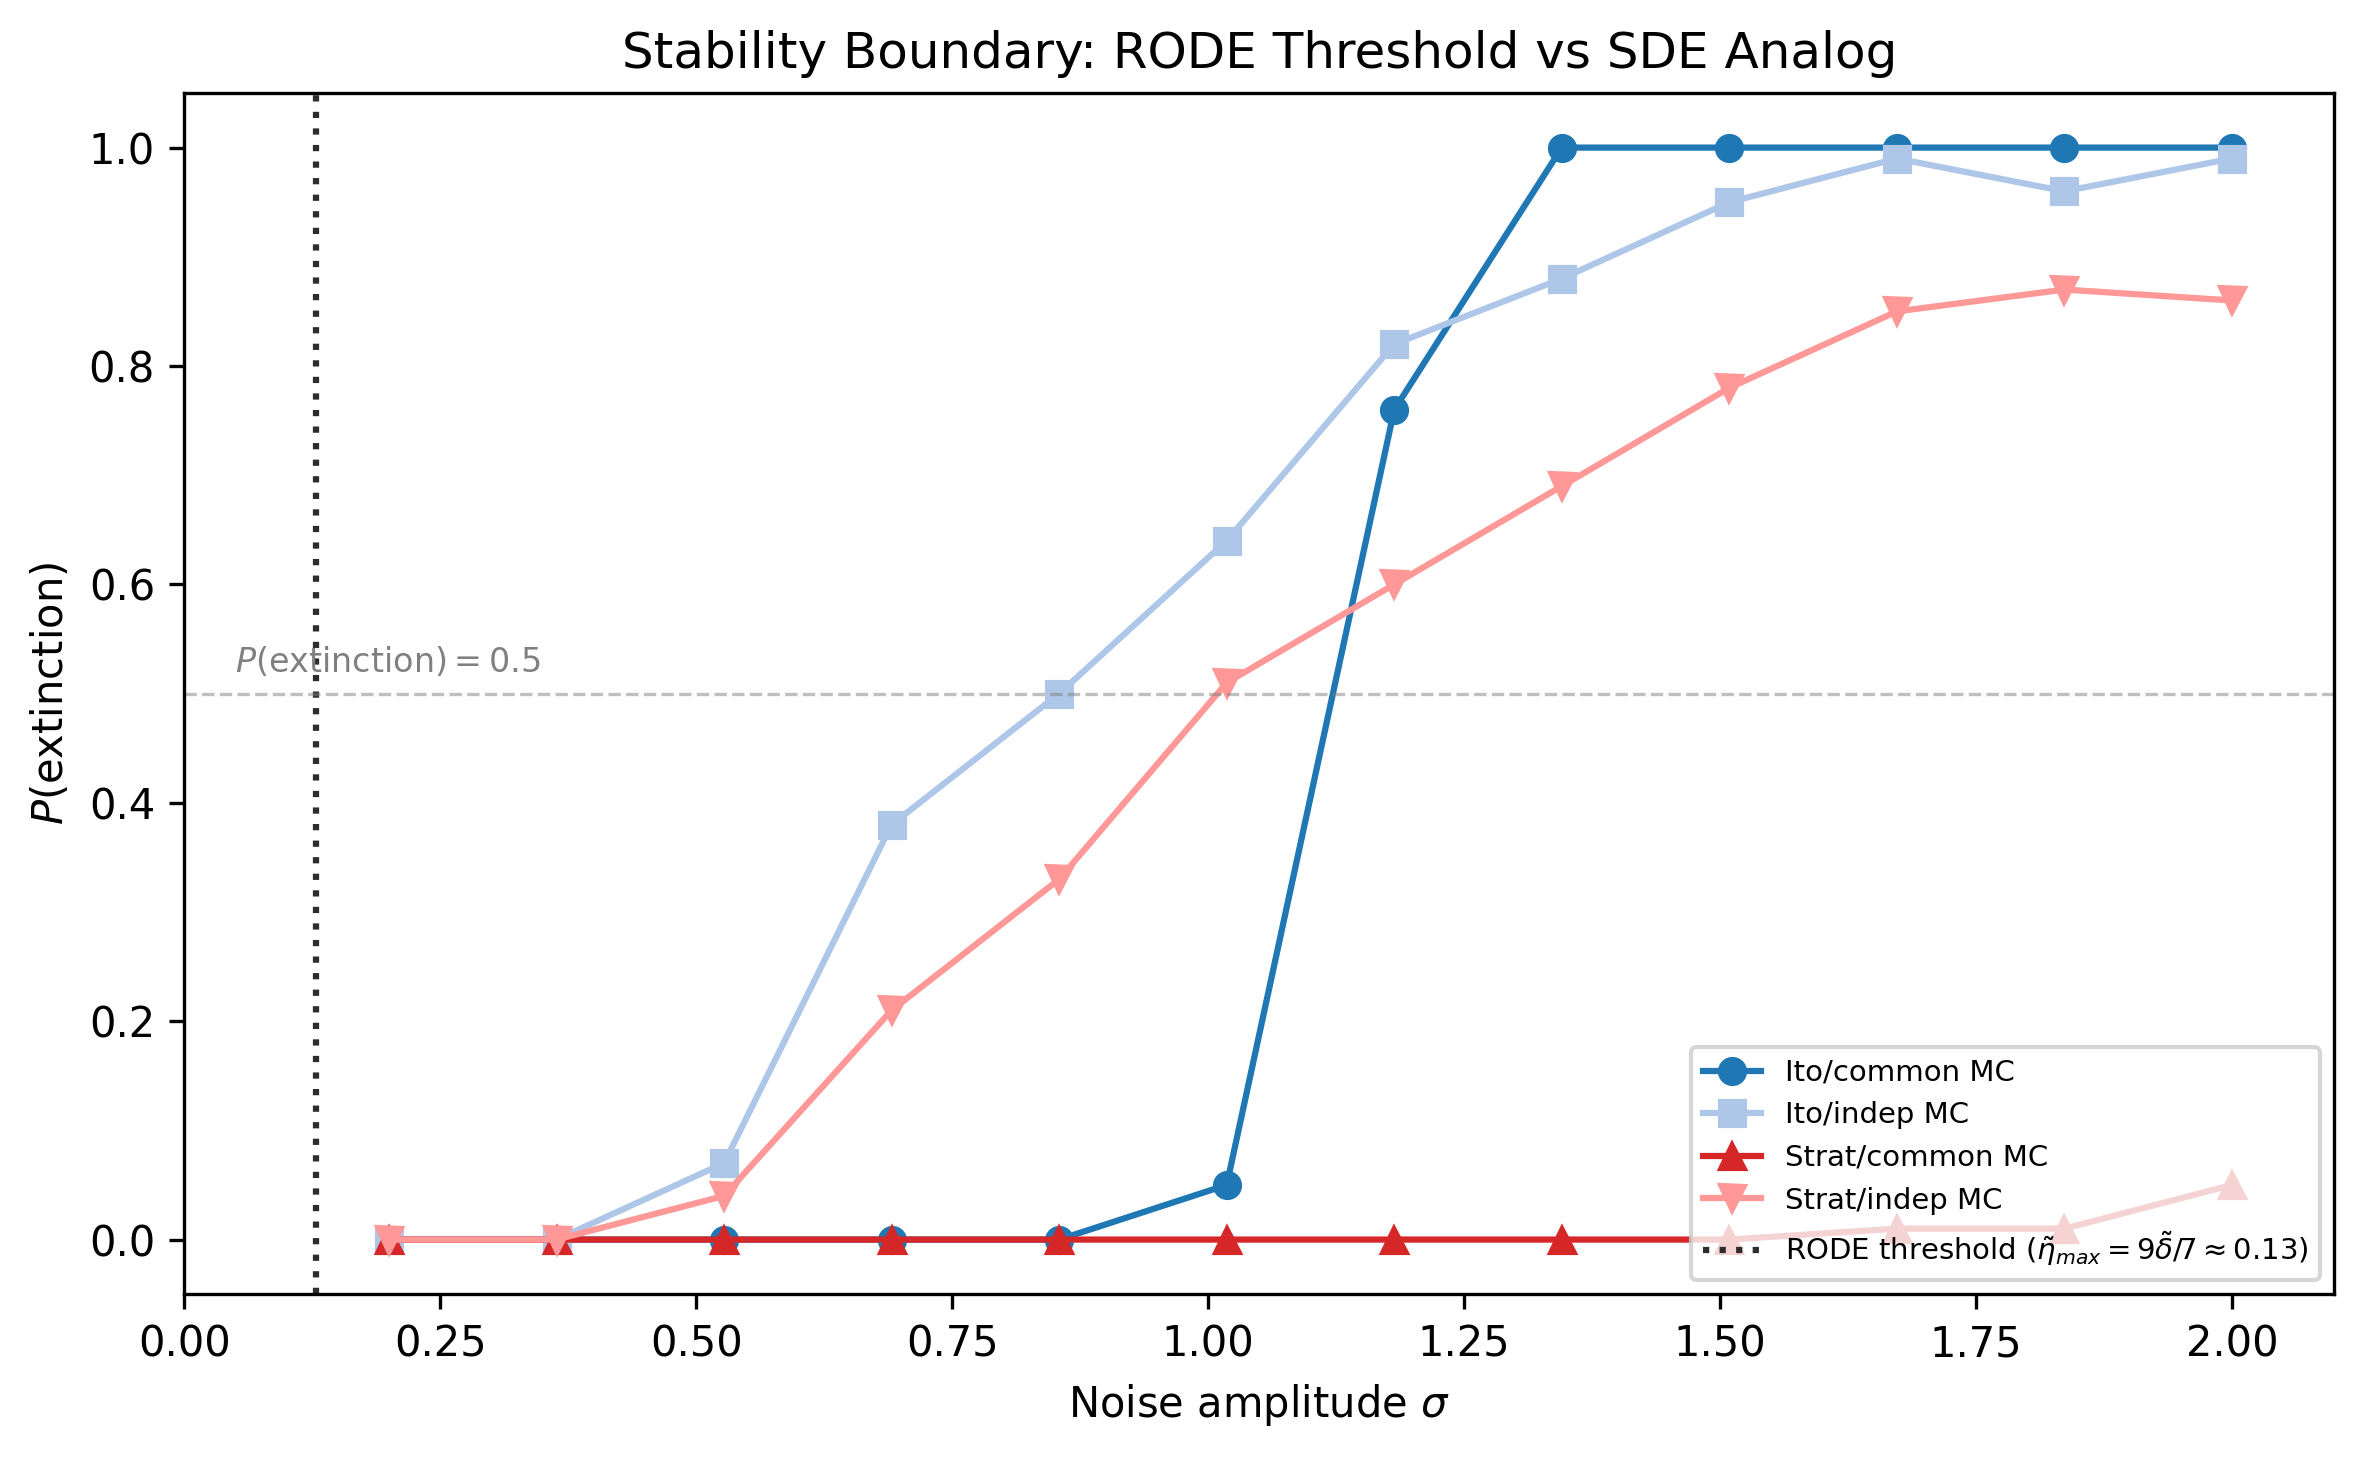
\includegraphics[width=\linewidth]{../poecilia_sde/figures/fig08_stability_boundary.png}

      \vspace{0.2cm}
      \renewcommand{\arraystretch}{1.1}
      \begin{tabular}{llc}
        \toprule
        Formulation & Noise & Boundary $\sigma$ \\
        \midrule
        RODE       & ---    & $\tilde\eta_{\max}\approx 0.13$ \\
        It\^{o}    & Common & $\sigma\approx 1.12$ \\
        It\^{o}    & Indep. & $\sigma\approx 0.86$ \\
        Strat.     & Common & $>2.0$ (not reached) \\
        Strat.     & Indep. & $\sigma\approx 1.01$ \\
        \bottomrule
      \end{tabular}
    \end{column}

    \begin{column}{0.4\textwidth}
      \textbf{RODE and SDE thresholds are 
      analytically non-equivalent.}

      \vspace{0.2cm}
      They measure fundamentally 
      different things:

      \vspace{0.2cm}
      \textbf{RODE:} phase-space contraction 
      at the population ceiling 
      (Liouville / boundary dissipativity)

      \vspace{0.2cm}
      \textbf{SDE:} linearized growth rate 
      of $\ln p$ near extinction 
      (scalar Lyapunov exponent)

      \vspace{0.2cm}
      \textcolor{alertred}{\textbf{Direct comparison is ill-posed.} 
      Translating a RODE threshold 
      into an SDE amplitude is 
      mathematically undefined.}
    \end{column}
  \end{columns}

\end{frame}

%%-------------------------------------------------
\section{Methodological Argument}
\stepcounter{subsection}
%%-------------------------------------------------

%%-------------------------------------------------
%% SLIDE 19: The Problem in the Literature
%%-------------------------------------------------
\begin{frame}{Single-Formulation Reporting: A Scientific Honesty Problem}
  \footnotesize

  \begin{alertblock}{A pattern in the stochastic modeling literature}
    A researcher studies a population system with stochastic environmental
    forcing.  The biological noise mechanism is not fully characterized from
    field data.  The researcher chooses one stochastic formulation ---
    often It\^{o}, because numerical libraries default to it --- runs
    simulations, and reports extinction probabilities or stability boundaries
    as findings.\\[6pt]
    \textbf{No justification is given for the formulation choice.\\
    No competing formulations are tested.\\
    The reported numbers are presented as evidence.}
  \end{alertblock}

  \vspace{0.3cm}
  This is \textbf{not} a minor technical oversight. It is a form of
  \textbf{selective reporting}: the researcher is presenting one answer
  from a family of plausible models without disclosing that the family
  exists.

  \vspace{0.2cm}
  In this system: the It\^{o} stability boundary is $\sigma\approx 1.12$;
  the Stratonovich/common boundary is $\sigma > 2.0$.  These are
  \textbf{qualitatively different conclusions} about when noise stabilizes
  the system.

\end{frame}

%%-------------------------------------------------
%% SLIDE 20: When Formulations Agree and Disagree
%%-------------------------------------------------
\begin{frame}{Robustness vs.\ Sensitivity: What Is Formulation-Dependent?}

  \begin{columns}[T]
    \begin{column}{0.5\textwidth}
      \begin{block}{Formulation-\textbf{robust} results}
        \begin{itemize}
          \item Discrimination speed $v$ governs extinction vs.\ coexistence in all five formulations
          \item Slow $v$ $\Rightarrow$ extinction; fast $v$ $\Rightarrow$ coexistence \emph{qualitatively} across all cases
          \item This ecological conclusion is not an artifact of formulation choice
        \end{itemize}
      \end{block}
    \end{column}

    \begin{column}{0.5\textwidth}
      \begin{alertblock}{Formulation-\textbf{sensitive} results}
        \begin{itemize}
          \item Stability boundary $\sigma$ differs significantly across formulations
          \item Extinction probability estimates diverge
          \item Mean trajectories differ (It\^{o} $\neq$ Stratonovich)
          \item RODE dissipativity threshold has no SDE analog
          \item Noise-induced mean shift: Stratonovich only
        \end{itemize}
      \end{alertblock}
    \end{column}
  \end{columns}

  \vspace{0.4cm}
  \begin{center}
    \textbf{Rule of thumb:} qualitative ecological conclusions may be robust;\\
    quantitative predictions for policy or management are not.
  \end{center}

\end{frame}

%%-------------------------------------------------
%% SLIDE 21: What Data Would Discriminate?
%%-------------------------------------------------
\begin{frame}{What Data Would Discriminate Between Formulations?}
  \footnotesize

  \begin{tabular}{p{4.8cm}p{5.5cm}}
    \toprule
    \textbf{Formulation choice} & \textbf{Discriminating data needed} \\
    \midrule
    \textbf{It\^{o} vs.\ Stratonovich} &
      Correlation time $\tau_c$ of environmental noise. \\
    \textit{If $\tau_c \to 0$: Stratonovich (Wong-Zakai).
      If $\tau_c$ large: RODE more appropriate.} &
      \textit{Measurable from hydrological records.} \\
    \midrule
    \textbf{Common vs.\ independent noise} &
      Cross-correlation of population fluctuations. \\
    \textit{If $\mathrm{Corr}(\delta f, \delta p) \approx 0$: independent.} &
      \textit{Measurable from multi-year census data.} \\
    \midrule
    \textbf{Displacement coefficient $c$} &
      Sperm volume transferred per encounter type. \\
    \textit{Riesch (2008) partial data: $c < 1$ likely.
      Requires controlled lab $+$ field experiment.} &
      \\
    \bottomrule
  \end{tabular}

  \vspace{0.3cm}
  \textbf{The modeling framework makes testable predictions.}\\
  The choice of formulation is not arbitrary --- it is a hypothesis.

\end{frame}

%%-------------------------------------------------
\section{Conclusions}
\stepcounter{subsection}
%%-------------------------------------------------

%%-------------------------------------------------
%% SLIDE 22: Summary of Findings
%%-------------------------------------------------
\begin{frame}{Summary}

  \begin{enumerate}
    \item[(a)] \textbf{Discrimination speed $v$ governs extinction/coexistence}
      across all five formulations --- a robust ecological finding independent
      of stochastic framework choice.

    \vspace{0.2cm}
    \item[(b)] \textbf{RODE boundary dissipativity} ($\eta_f+\eta_m+\eta_p < 3$)
      characterizes phase-space contraction at the carrying capacity.
      The Stratonovich Lyapunov exponent is noise-amplitude independent;
      the It\^{o} exponent is shifted by $-\sigma^2/2$.

    \vspace{0.2cm}
    \item[(c)] \textbf{Formulation determines mean behavior:}
      It\^{o} noise does not shift ensemble means (martingale property);
      Stratonovich noise adds an effective birth rate increment
      $+\tfrac{1}{2}\sigma_i^2\,\E[u_i]$ --- largest for the parasite.

    \vspace{0.2cm}
    \item[(d)] \textbf{Under independent multiplicative noise,}
      diffusion cross-driving between populations vanishes at mean-field
      level; deterministic coupling still generates covariance through
      shared nonlinear drift.
  \end{enumerate}

\end{frame}

%%-------------------------------------------------
%% SLIDE 23: Take-Home Message
%%-------------------------------------------------
\begin{frame}{Take-Home Message}

  \footnotesize

  \begin{alertblock}{On this biological system}
    Noise can save the sperm parasite --- but \emph{which} noise,
    formulated \emph{how}, determines whether it does so by shifting
    the mean trajectory (Stratonovich) or by suppressing growth variance
    (It\^{o}).  These are different mechanisms with different empirical
    signatures.
  \end{alertblock}

  \vspace{0.3cm}
  \begin{block}{On mathematical modeling practice}
    When the biological phenomenon is not fully characterized,
    choosing a single stochastic formulation and presenting its
    quantitative predictions as evidence is \textbf{scientifically
    dishonest}.\\[6pt]
    The minimum standard is: state your formulation, justify it
    biologically, and test the sensitivity of your conclusions
    to competing formulations.\\[6pt]
    \textbf{Robustness to formulation choice is a result, not an assumption.}
  \end{block}

\end{frame}

%%-------------------------------------------------
%% SLIDE 24: Thank you
%%-------------------------------------------------
\begin{frame}{Thank you for your attention}


  \vspace{0.3cm}
  \begin{columns}[T]
    \begin{column}{0.25\textwidth}
      
\includegraphics[width=\linewidth]{../figures/QR_biomathematicus.png}
    \end{column}
    \begin{column}{0.75\textwidth}
      \vspace{0.3cm}
      \textbf{Juan B.\ Gutiérrez}\\
      \texttt{juan.gutierrez3@utsa.edu}\\
      \textsc{University of Texas at San Antonio}\\[6pt]
      %\footnotesize Manuscript available via QR code.
    \end{column}
  \end{columns}

\end{frame}


\end{document}
